% Když budete cokoli psát: ukládejte starší verze vždy odděleně, abyste se 
% k nim mohli kdykoli vrátit. Kusy textu, které jste se rozhodli nepoužít, taky ukládejte do zvláštního souboru. Smazat se to dá vždycky, ale psát to znova je opruz. 

% A POŘÁD ZÁLOHUJTE. POŘÁD !!!

\documentclass[12pt, a4paper, oneside]{article} 
% velikost písma, stránky, typ dokumentu -- detaily viz literatura

%\usepackage{czech} % nastavení češtiny
%\usepackage[latin2]{inputenc}
%\usepackage[cp1250]{inputenc} % pro win1250
\usepackage[center]{caption} 
\usepackage[utf8]{inputenc}
\usepackage{wrapfig} % nastavení obtékání textu
\usepackage{graphicx,amsmath} % nastavení grafiky, matematiky
\usepackage{subfig} % více obrázků vedle sebe 
\usepackage{float}
\usepackage{amsmath}
\usepackage{amssymb}
\usepackage{bbding}
\usepackage{enumitem}
\usepackage{breakurl}
\usepackage{pdflscape}

%\usepackage{indentfirst}

\usepackage{tocloft} %přidá tečky do obsahu ke kapitolám /sekcím 
\renewcommand{\cftsecdotsep}{\cftdotsep}

\usepackage[bookmarksopen,colorlinks,plainpages=false,linkcolor=black,urlcolor=blue,citecolor=black,filecolor=black,menucolor=black,unicode=true]{hyperref}

\urlstyle{rm}
%bookmarksopen -- open up bookmark tree 
%colorlinks -- zbarví odkazy (implicitně orámovaný nezbarvený text)
%urlcolor -- barva odkazů (implicitně magenta) 
%linkcolor=black -- barva odkazů v obsahu (implicitně red)


\usepackage{listings}
\usepackage{color}
\usepackage{minted}
\definecolor{lightgray}{RGB}{240,240,240}
\definecolor{darkgray}{rgb}{.4,.4,.4}
\definecolor{purple}{rgb}{0.65, 0.12, 0.82}
\definecolor{darkgreen}{RGB}{0,150,0}

\usemintedstyle{perldoc}
\newminted{js}{linenos=true, bgcolor=lightgray}

\lstdefinelanguage{JavaScript}{
  keywords={typeof, new, true, false, catch, function, return, null, catch, switch, var, if, in, while, do, else, case, break, for},
  keywordstyle=\color{blue}\bfseries,
  ndkeywords={class, export, boolean, throw, implements, import, this},
  ndkeywordstyle=\color{blue}\bfseries,
  identifierstyle=\color{black},
  sensitive=zr,
  comment=[l]{//},
  morecomment=[s]{/*}{*/},
  commentstyle=\color{darkgreen}\ttfamily,
  stringstyle=\color{red}\ttfamily,
  morestring=[b]',
  morestring=[b]"
}

\lstset{
   backgroundcolor=\color{lightgray},
   extendedchars=true,
   basicstyle=\footnotesize\ttfamily,
   showstringspaces=false,
   showspaces=false,
   numbers=left,
   numberstyle=\footnotesize,
   numbersep=9pt,
   tabsize=2,
   breaklines=true,
   showtabs=false,
   aboveskip=5mm,
   belowskip=7mm,
   captionpos=b
}

\renewcommand{\listingscaption}{Example}
\renewcommand{\listoflistingscaption}{Code samples}

% \usepackage{parskip} -- zapne americké odstavce v celé práci

\addtolength{\textwidth}{-2mm} 
\addtolength{\hoffset}{4mm}  % posun textu kvůli kroužkové vazbě  

\setlength{\intextsep}{5mm} % nastavení mezery okolo obrázků

% nastavení příkazu >\figcaption pro popis čehokoli, jako by to byly obrázky 
\makeatletter   
\newcommand\figcaption{\def\@captype{figure}\caption}
\makeatother

\renewcommand\refname{References} 
%\def\bibname{PŘÍLOHA D: Reference}
%\renewcommand\bibname{PŘÍLOHA D: Reference}
% přejmenuje anglický název Reference na české Literatura


%\makeindex % příprava pro výrobu indexu (jestli ho chcete)

%%    VLNKA <fileinput>  KkSsVvZzOoUuAaIi        
% Defaultni  koncovka pro <fileinput> je  ".tex"
%FIXME: haze error
%\cstieon % Vypne chovani vlnky jako tvrde mezery v matematickem rezimu

%%%%%%%%%%%%%%%%%%%%%%%%%%%%%%%%%%%%%%%%%%%%%%%%%%%%%%%%%%%%%%%
%V PROSTŘEDÍ ROVNIC SE NESMÍ VYSKYTOVAT PRÁZDNÝ ŘÁDEK
%
%PROGRAMY VLNKA A CSINDEX SE MUSÍ SPUSTIT SAMOSTATNĚ
%%%%%%%%%%%%%%%%%%%%%%%%%%%%%%%%%%%%%%%%%%%%%%%%%%%%%%%%%%%%%%%

% definice příkazů 
\newcommand{\D}{\medskip \noindent} % nový odstavec v "americkém" formátování 
\newcommand{\B}{\textbf} %tučné písmo
\newcommand{\A}{\mathbf} %tučné písmo v matematickém režimu
\newcommand{\TO}{\ensuremath{\boldsymbol\Omega}} % tučný znak velké omega -- pro ohmy
\newcommand{\I}{\index}  % vytváří položku indexu (asi nepoužijete)
\newcommand{\Deg}[1][]{\ensuremath{{#1}^\circ}} % vysází značku stupně Celsia
\newcommand{\Def}{\footnotesize Definice: \normalsize}
\newcommand{\Pos}{\footnotesize Experiment: \normalsize}
\newcommand{\Odv}{\footnotesize Odvození: \normalsize}
\newcommand{\Vym}{\footnotesize Vymezení pojmu: \normalsize}
\newcommand{\Ob}{image }
\newcommand{\It}{\textit}  % kurzíva
\newcommand{\M}{\mathrm}   % v prostředí rovnic nastaví normální písmo (místo kurzívy ) 
\newcommand{\F}{\footnotesize} % zmenšená velikost písma
\newcommand{\N}{\normalsize} % normální velikost písma
%\newcommand{\U}{\underline}  % podtržené písmo
\newcommand{\e}{\ensuremath} 
\newcommand{\Has}{\textcolor{green}{\CheckmarkBold}}
\newcommand{\NoHas}{\textcolor{red}{\XSolidBrush}}
% další příkaz se aplikuje, pouze, když jste v matematickém režimu

%\hyphenation{Pusť-me pla-tí hod-no-ty do-sa-dí-me za-da-né dal-ším}
% dělení slov, kdyby implicitní nevyhovovalo

\linespread{1.3} 
% řádkování 1,5x  
% použijete podle situace  

\unitlength=1mm % nastavení volby jednotek 

% konec hlavičky
%%%%%%%%%%%%%%%%%%%%%%%%%%%%%%%%%%%%%%%%%%%%%%%%%%%%%%%%%%%%%%%%%%%
%%%%%%%%%%%%%%%%%%%%%%%%%%%%%%%%%%%%%%%%%%%%%%%%%%%%%%%%%%%%%%%%%%%

\begin{document} % začátek textové části 

% titulní strana
\pagestyle{empty} % vynechá číslování
 
\voffset = -20mm % posun začátku textu výš
\enlargethispage{60mm} % zvětší oblast tisku pro tuto stránku   

\begin{center}
 
\Large \B{STŘEDOŠKOLSKÁ ODBORNÁ ČINNOST}

\vspace{60mm}

\huge %\LARGE
\B{LORRIS TOOLBOX \\ Set of tools for developement and control of robots}
% na titulní straně může být stručnější, pokud je to potřeba  

\Large

\vspace{90mm}


\B{Vojtěch Boček} \\

\vspace{40mm}

\B{Brno 2013}


\end{center}

\newpage % konec titulní strany 
%%%%%%%%%%%%%%%%%%%%%%%%%%%%%%%%%%%%%%%%%%%%%%%%%%%%%%%%%%%%%%%%%%%%%%%%%%%

% vnitřní titulní strana
\voffset = -20mm % posun začátku textu výš
\enlargethispage{60mm} % zvětší oblast tisku pro tuto stránku   

\begin{center}

\Large \B{STŘEDOŠKOLSKÁ ODBORNÁ ČINNOST}  \\
\vspace{10mm}
 \normalsize 
\B{Obor SOČ: 18. Informatika}% číslo a název -- vyplníme spolu 

\vspace{45mm}

\LARGE %\huge 
\B{LORRIS TOOLBOX \\ Set of tools for developement and control of robots} 
\end{center}  
\large

\vspace{50mm}


\begin{tabbing}
\hspace{10mm} \= \hspace{30mm}  \=   \kill % nastavení zarážek 
  \> \B{Author:}  \> \B{Vojtěch Boček}        \\[8mm] 
  \> \B{School:}   \> \B{SPŠ a~VOŠ technická, }     \\
  \>              \> \B{Sokolská 1, 602 00 Brno}    \\[8mm]

  \> \B{Consultant:} \> \B {Jakub Streit} 
\end{tabbing}

\vspace{20mm}

\begin{center}
\B{Brno 2013}

\end{center}
\normalsize

%%%%%%%%%%%%%%%%%%%%%%%%%%%%%%%%%%%%%%%%%%%%%%%%%%%%%%%%%%%%%%%%%%%%%%%%%%%
\newpage   % Poděkování -- nepovinné 
\voffset = 0mm % posun začátku textu zpět

~ % musí to tu být, aby fungovala svislá mezera
\vspace{100mm}

\section*{Acknowledgement}
Thanks to Jakub Streit for his advices, help, and much patience he provided during my work on this project, to Martin Vejnár for his Shupito programmer, to Mgr. Miroslav Burda for great help with text part of this work and last but not least, to Bc. Martin Fouček for his advices and help with Qt Framework. Thanks goes also to DDM Junior for their support.

\D This work was made with financial support from JMK a JCMM.

\begin{figure}[H]
\begin{center}

\includegraphics[width=\textwidth]{img/jcmm.png}
\end{center}
\end{figure}
 

%%%%%%%%%%%%%%%%%%%%%%%%%%%%%%%%%%%%%%%%%%%%%%%%%%%%%%%%%%%%%%%%%%%%%%%%%%%
\newpage   % Anotace 
~ % musí to tu být, aby fungovala svislá mezera
\vspace{10mm}

\section*{Annotation}

This work describes a~complex set of tools designed for developement and control of any device capable of connecting to serial port or TCP socket.

Because Lorris isn't a~simple application nor is it a~toolbox focused on one narrow area of use, because the whole set is continuously growing and because scope of use for all features and modules of Lorris is too big, it is impossible to briefly describe it all in limited scope of annotation.

To get better notion of what can one achieve with Lorris, please refer to introductory chapter of this work (English version of this text is available on enclosed CD as PDF file).

Main asset of this software package is the ability to significantly speed-up and simplify developement and testing of various applications for microcontrollers, typically programming and controlling various kinds of robots.

\D \B{Key words:} binary data analysis, programming and control of robots, developement for microcontrollers, programming of microchips

\addtolength{\textheight}{30mm} % prodlouží následující stránku

%%%%%%%%%%%%%%%%%%%%%%%%%%%%%%%%%%%%%%%%%%%%%%%%%%%%%%%%%%%%%%%%%%%%%%%%%%%
\newpage
\pagestyle{plain}

\setlength{\voffset}{-20mm} % posune text/obrázek na této stránce nahoru
\setcounter{page}{1}  % nastaví čítač stránek znovu od jedné

\tableofcontents  % vysází obsah

\addtolength{\textheight}{-30mm} % zkrátí následující stránku
%%%%%%%%%%%%%%%%%%%%%%%%%%%%%%%%%%%%%%%%%%%%%%%%%%%%%%%%%%%%%%%%%%%%%%%%%%%
\newpage
\setlength{\voffset}{0mm} % posune text/obrázek na této stránce, kam patří
%\pagestyle{headings} % znovu zapne číslování
\pagestyle{plain}


\section*{Introduction}
\addcontentsline{toc}{section}{Introduction}
Lorris is extensive set of tools which all share the same goal -- to help with development, debugging and control of electronic devices, mainly robots. This chapter briefly describes the most important features of all modules and each module is throughly described in it's own chapter further on.

\subsection*{Module: analyzer}
\addcontentsline{toc}{subsection}{Module: analyzer}
\begin{itemize}
    \item Its main purpose is to graphically display data from the device.
    \item Analyzer uses widgets to display data -- small "windows", each showing certain part of data.
    \item Each widget has individual settings and the user can place them anywhere on the workspace.
    \item Thanks to widgets, it is possible to assemble interface suitable for virtually any device.
    \item Several types of widgets are available in Lorris, for example \It{Number, Color, Column bar, Circle} (displaying angle within circle) or \It{Graph}.
    \item Analyzer is also ideal for easy displaying of data from components for which using only numbers is not eligible, e.g. color sensor.
    \item Some widgets can also send data to the device. Consequently, it means that beside displaying data, widgets can also control the device.
    \item Of all the widget types, \It{Script} is the most notable one. The user writes his own script, which processes the incoming data. User's script can use other widgets and other parts of Lorris, which means that it can display or in other ways interpret virtually any data.
    \item Using script, the user can modify the behavior of Lorris itself.
\end{itemize}

\subsection*{Module: programmer}
\addcontentsline{toc}{subsection}{Module: programmer}
\begin{itemize}
    \item Graphical interface for several types of bootloaders and programmers of microchips.
    \item It can write program to chip, read and erase chip's memory or program chip's fuses.
    \item Official GUI for Shupito programmer.
    \item Shupito is microchip programmer. One end goes to computer, the other one to the chip -- you need programmer to program some types of chips.
\end{itemize}

\subsection*{Module: terminal}
\addcontentsline{toc}{subsection}{Module: terminal}
\begin{itemize}
    \item Regular terminal -- displays incoming data either as text or as hexadecimal byte dump.
\end{itemize}

\subsection*{Module: proxy between serial port and TCP socket}
\addcontentsline{toc}{subsection}{Module: proxy between serial port and TCP socket}
\begin{itemize}
    \item Proxy creates server connected to serial port. The serial port is then accessible from anywhere via the internet.
    \item It makes it possible to debug, control or otherwise communicate with the device via internet network.
\end{itemize}
~
\vspace{10mm}

\noindent\It{Enclosed CD contains promotional poster as PDF file.}

\newpage
\section{Motivation}
\label{motivace}
I'm a member of one of the teams which build robots for various competitions, and I've met a problem while we were building one of our robots -- such robot usually contains a pretty large number of various sensors (ultrasound range meters, encoders for measuring covered distance, buttons which detect collision with borders of the game field ...), and there was no way to show data from those sensors comfortably and clearly.

In order to simplify and speed-up development of the robot, I decided to find some computer application which would show data from the robot in clear and well-arranged manner. Requirements which I set for this application are specified in chapter \ref{reqs}.

\subsection{Requirements for application}
\label{reqs}
%\addcontentsline{toc}{subsection}{Requirements for application}
I require following features from the application:
\begin{enumerate}
    \item Ability to process data from device and show them clearly % 1
    \item Support for many formats of incoming data% 2
    \item Quick and simple to use% 3
    \item Support for other operating systems than MS Windows % 4
    \item Low price% 5
    \item Ability to easily expand program, ideally open-source % 6
    \item No dependencies on other applications (eg. MS Office Excel) % 7
\end{enumerate}

\subsection{Present applications}
%\addcontentsline{toc}{subsection}{Present applications}
I've found only several programs which have at least similiar function (reading data from serial port and displaying them). Basically only two types of applications are available -- commercial, which cost a lot of money (and still don't meet all the requirements) or applications which can display data in only one format, typically in graph.

\begin{itemize}
    \item {\bf SerialChart}\cite{serialchart} is open-source program\footnote{Program with publicly available source code, free to modify and use} which can parse and display data from serial port. SerialChart is simple and well arranged, but it can display data only in graph and it is configured by hand-written configuration file.
    \item {\bf WinWedge}\cite{winwedge} is commercial program. It can process data from serial port and display them as a graph in MS Excel or as a web page. It can also send commands back to connected device, but it has bad user interface and the need for another program (like MS Excel) to actually show the data is not ideal. It is available only for MS Windows and basic version costs \$ 259.
    \item {\bf Advanced Serial Data Logger}\cite{serialdatalogger} is designed to be used primarily to collect data from serial port and export them, thus you have to use another application to display the data (eg. MS Excel), similarly to WinWedge.
    \item {\bf StampPlot Pro}\cite{stamplot} can process incoming data in widgets created by user, but it is not simple to use, it is not open-source, it is available only for MS Windows and I haven't managed to get it working under Windows 7.
    \item {\bf LabVIEW}\cite{labview} is very large software package with long history and is is possible to use it for wide variety of operations -- various laboratory measurements, analysis of data signals, controlling of robots, controlling of whole systems for laboratory measurements and much more. However, LabVIEW is closed proprietary software and because of its specialization, it is also very expensive. Basic license costs about \$~1150.
\end{itemize}

\subsection{Comparison of applications}
%\addcontentsline{toc}{subsection}{Comparison of applications}
Following table lists features of each application. Numbering of requirements matches the list in chapter "Requirements for application".

\vspace{5mm}

\begin{tabular}{ | l | l | l | l | l | l | l | l |}
    \hline
    Requirements                & 1      & 2      & 3      & 4      & 5      & 6      & 7      \\ \hline
    SerialChart                 & \Has   & \NoHas & \Has   & \NoHas & \Has   & \Has   & \Has   \\ \hline 
    WinWedge                    & \NoHas & \Has   & \Has   & \NoHas & \NoHas & \NoHas & \NoHas \\ \hline 
    Advanced Serial Data Logger & \NoHas & \Has   & \Has   & \NoHas & \NoHas & \NoHas & \NoHas \\ \hline 
    StampPlot Pro               & \Has   & \Has   & \NoHas & \NoHas & \Has   & \NoHas & \Has   \\ \hline 
    LabVIEW                     & \Has   & \Has   & \NoHas & \Has   & \NoHas & \NoHas & \Has   \\ \hline
%    Lorris                      & \Has   & \Has   & \Has   & \Has   & \Has   & \Has   & \Has   \\ \hline 
\end{tabular}

\vspace{5mm}

I've decided to write my own program which will meet all the requirements because no such application exists.

\section{Lorris}
Lorris is a program written in C++ with use of Qt Framework\cite{qtfrm}. Qt is multiplatform framework, which (among other things) makes it possible to run Lorris on multiple operating systems -- I'm using Debian Linux\cite{debian} (Wheezy, 64bit) and Windows 7 for testing.

\subsection{Website and repository}
Lorris' GIT\footnote{\It{GIT} -- distributed version control system} repository is hosted on GitHub\cite{github}. GitHub also provides hosting for project's website, which contains links to prebuilt Lorris binaries for Windows, description of program, video introduction to Lorris (6 min.), screenshots of Lorris and information how to build Lorris under MS Windows and Linux.
\begin{itemize}
    \item Repository: \url{https://github.com/Tasssadar/Lorris}
    \item Website (Czech):\\ \url{http://tasssadar.github.com/Lorris/cz/index.html}
    \item Website (English):\\ \url{http://tasssadar.github.com/Lorris/index.html}
    \item SOČ presentation: \\ \burl{http://www.sokolska.cz/soc-2012/bocek-vojtech-lorris-sada-nastroju-pro-robotiku/}
\end{itemize}
There is still an ongoing developement in application's repository.

\subsection{Application's structure}
The program is designed as modular application, so that it can accommodate several parts which, although they are separate, share the same area of use.
Base part of application provides connection to device (e.g. to robot or to development board with chip), tab-based user interface and storage for application settings, but data processing itself takes place in individual modules.

Modules are opened as tabs, much alike pages in web browser. Lorris can open several windows at once and it can split each window to multiple parts like presented in image \ref{split_img} -- window is divided in the middle, you can see two tabs at once. The one on the left is analyzer and the other one is terminal. \\
\\
\noindent Connection options:
\begin{itemize}
    \item Serial port
    \item Shupito Tunel (virtual serial port, more in chapter \ref{tunel})
    \item TCP socket\footnote{\It{Transmission Control Protocol} -- connection via internet.}
    \item Loading data from file
\end{itemize}
It is possible to connect multiple modules to one device.

\begin{figure}[H]
\begin{center}
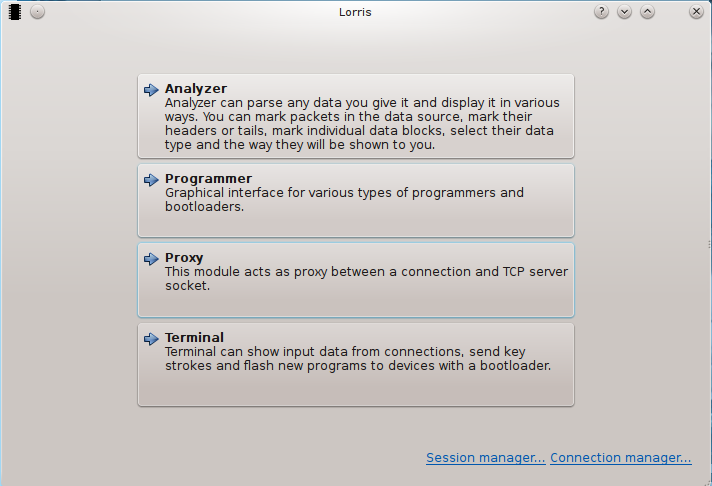
\includegraphics[scale=0.6]{img/new_tab.png}
\caption{Tab creation dialog}
\end{center}
\end{figure}

\begin{figure}[H]
\begin{center}
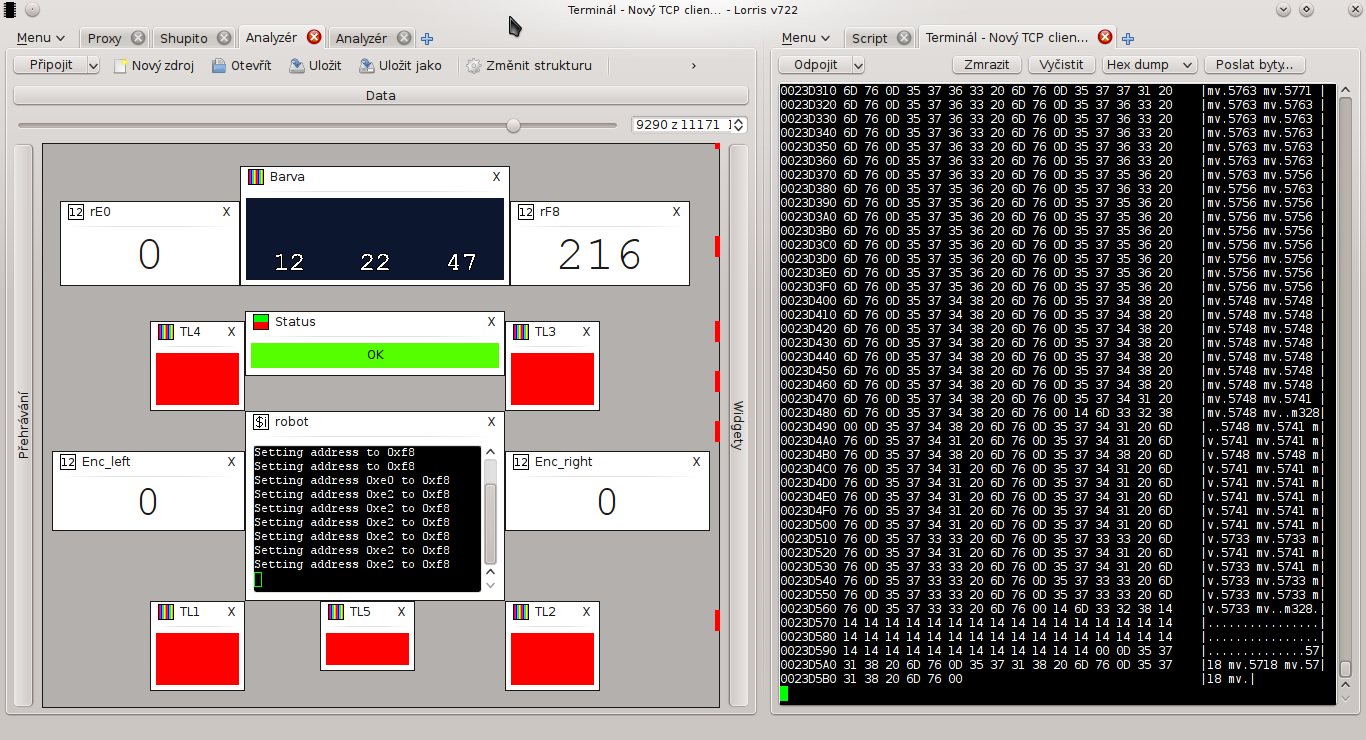
\includegraphics[width=\textwidth]{img/split.png}
\caption{Window divided to multiple parts}
\label{split_img}
\end{center}
\end{figure}

\enlargethispage{60mm} % zvětší oblast tisku pro tuto stránku   
\setlength{\voffset}{-20mm}
\addtolength{\textheight}{20mm}
\newpage
\subsection{Session}
Lorris can save everything user opened (tabs, their layout, connection, data of each tab, ...) as session. User can later load saved session and thus return to his previous work. Lorris automatically saves session before it is closed, so when user starts Lorris again, all his work is in the same state as it was before he left.

\subsection{Automatic updates}
Lorris can update itself under MS Windows. It checks for new version on start, and if there is one available, it shows little notification:
\begin{figure}[H]
\begin{center}

\includegraphics[scale=1]{img/update_notify.png}
\caption{New update notification}
\end{center}
\end{figure}
In case user confirms the update, Lorris closes itself and runs little updater application. Updater shows changelog and downloads new version and installs it.
\begin{figure}[H]
\begin{center}
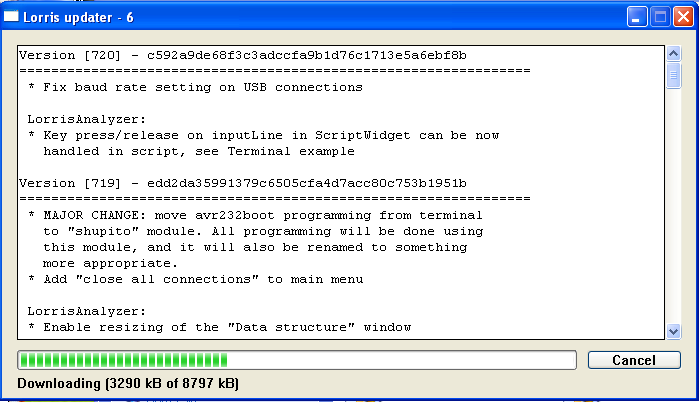
\includegraphics[scale=0.65]{img/updater.png}
\caption{Ongoing update}
\end{center}
\end{figure}

\setlength{\voffset}{0mm}
\addtolength{\textheight}{-20mm}
\newpage
\section{Module: Analyzer}

\begin{figure}[h]
\begin{center}
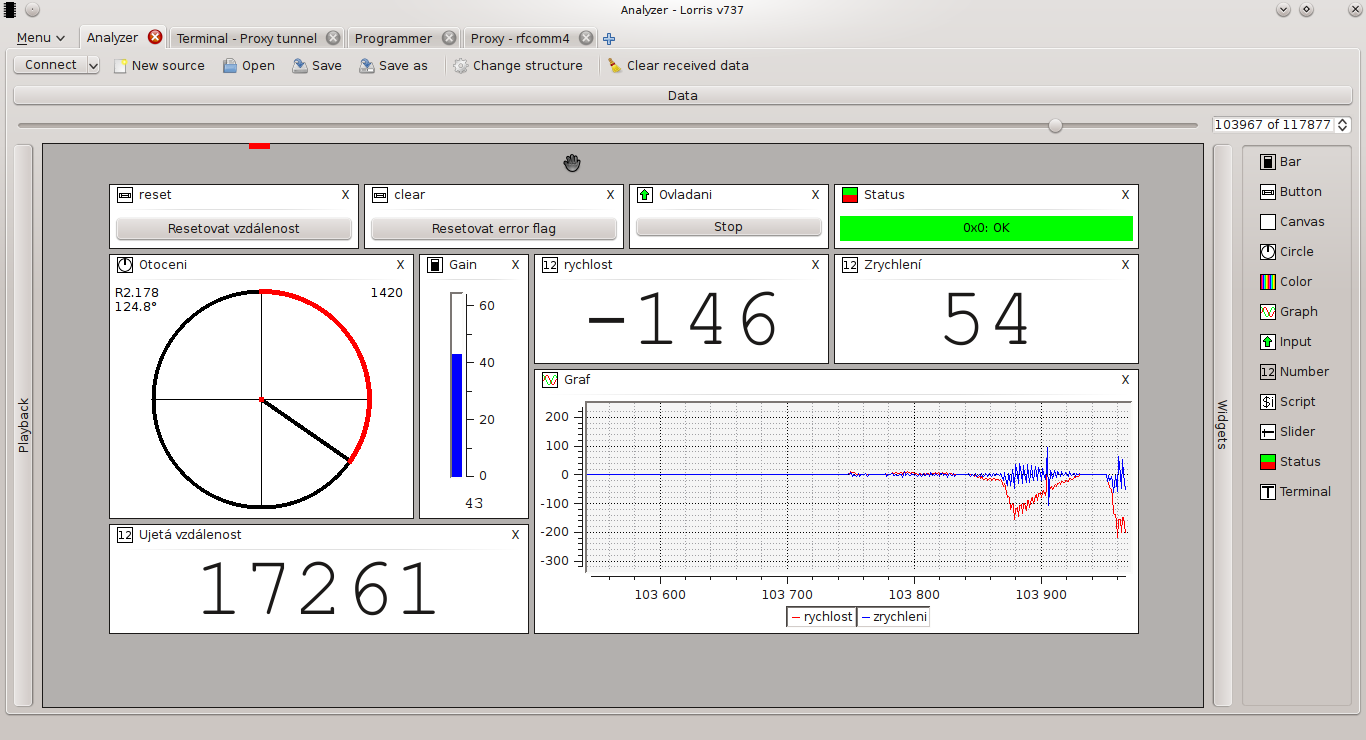
\includegraphics[width=\textwidth]{img/analyzer_all.png}
\caption{Module analyzer}
\label{Analyzer}
\end{center}
\end{figure}

This module parses incoming data (structured as packets) and displays them in graphical widgets. Application saves processed data into memory -- user can go through received packets using slider and textbox in upper part of the window. All data (received packets, packet structure and widgets positions and settings) can be saved to file. 

Packet structure is configured in dialog window (image \ref{Analyzer_struct}). It is possible to set packet's length, endianness\footnote{\It{Endianness} -- order of bytes in numbers}, packet's header and its content -- static data ("start byte"), dynamic lenght od packet and command and device ID. Packets can be later filtered by command or device ID.

\newpage
\setlength{\voffset}{0mm}
\pagestyle{plain}

Incoming data show up in upper part of the window when packet structure is set and user can then "drag" widgets from the list in right part of the window to workspace. Data are assigned to widget again using drag\&drop, this time user has to drag first byte of data to widget.

Widget then displays data from that byte (or several bytes if needed). Assigned byte is highlighted when user puts mouse over the widget, so that he can find out which data belong to which widget.

Widget settings are available in context menu under right-click. User can set title and other parameters different for each widgets -- these parameters will be described in each widget's section later. Widgets can also be locked, which means the widget can't be closed nor moved or resized.

It is possible to precisely position widgets using grid or by using "aligment lines" (see image \ref{widget_lines}). User can also easily clone widgets by moving them while holding the control key.

Some widgets might profit from following feature: if user grasps widget with mouse as if he wanted to move it and then "shakes it" from right to left, the widget will expand itself to cover all of the visible workspace. When it is moved, it will shrink to it's original size.

\begin{figure}[H]
\begin{center}
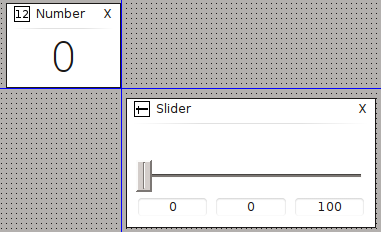
\includegraphics[scale=1]{img/lines.png}
\caption{Widget aligment using grid and lines}
\label{widget_lines}
\end{center}
\end{figure}

\begin{figure}[H]
\begin{center}
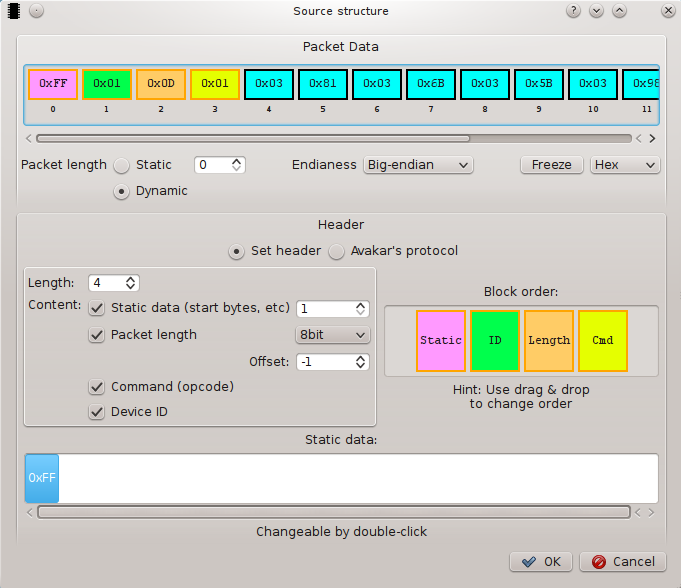
\includegraphics[scale=0.65]{img/analyzer_struct.png}
\caption{Packet structure dialog}
\label{Analyzer_struct}
\end{center}
\end{figure}

\enlargethispage{60mm} % zvětší oblast tisku pro tuto stránku   
\setlength{\voffset}{-25mm}
\addtolength{\textheight}{20mm}
\newpage
\begin{figure}[H]
\begin{center}
\subfloat[List of widgets]{\label{analyzer_widgets}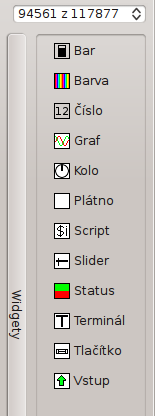
\includegraphics[scale=1]{img/analyzer_widgets_new.png}}
\hfill
\subfloat[Assigning data using drag\&drop]{\label{analyzer_widgets}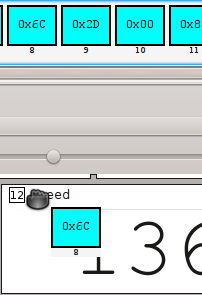
\includegraphics[scale=1]{img/analyzer_drag_data.png}}  
\caption{Widgety}
\label{widgets}
\end{center}
\end{figure}

\subsection{Filters}
Analyzer can filter incoming data and each filter may contain several conditions, which determine if packet is filtered out or not.
\begin{figure}[H]
\begin{center}
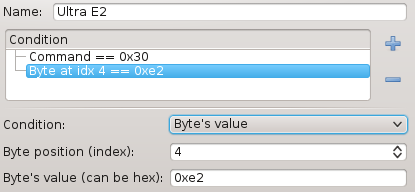
\includegraphics[scale=0.9]{img/filters.png}
\caption{Filter settings}
\end{center}
\end{figure}

\setlength{\voffset}{0mm}
\addtolength{\textheight}{-20mm}
\newpage
Each condition can check command or device ID from packet's header, value of byte in packet or  it can run simple user script. Thanks to the script, it is possible to write almost any kind of condition.

\begin{listing}[H]
\begin{jscode}
// Return true if passes, false if it
// should be filtered out
function dataPass(data, dev, cmd) {
    return false;
}
\end{jscode}
\caption{Script filter condition}
\end{listing}

% TODO: newpage
\subsection{Widget: number}
\begin{figure}[h]
\begin{center}
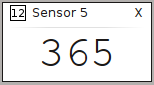
\includegraphics[scale=1]{img/w_num.png}
\caption{Widget: number}
\end{center}
\end{figure}
This widget displays integers (both signed and unsigned, 8 to 64bits) and decimal numbers (single-precision\footnote{Standard floating-point number format used in C and other languages (IEEE 754-2008)}, 32 and 64 bit).
Widget can align the number to max lenght of it's data type and format as follows:
\begin{itemize}
    \item Decimal -- number as base 10
    \item Decimal with exponent -- uses exponent to display big numbers, available only for decimal numbers
    \item Hexadecimal -- number as base 16, available only for unsigned numbers
    \item Binary -- number as base 2, available only for unsigned numbers
\end{itemize}

Another feature is option to recalculate widget's value using formula specified by the user. This is useful for example while showing data from infrared range finders, because their output value must be converted to centimeters using equasion. Formula can look like this:
\begin{center}
\verb|2914/(%n+5)-1|
\end{center}
where \verb|%n| is alias for number which would otherwise be displayed in the widget. This particular formula converts distance measured by Sharp GP2Y0A41 infrared range finder to centimeters.

\subsection{Widget: bar}
\begin{figure}[H]
\begin{center}
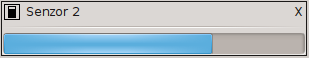
\includegraphics{img/w_bar.png}
\caption{Widget: bar}
\end{center}
\end{figure}
Data in this widget are displayed as bar. User can set data type (same as widget \It{number}), orientation (vertical or horizontal) and range of displayed values. It can also use formula to re-calculate it's value in the same way as widget \It{number}.

\subsection{Widget: color}
\begin{figure}[H]
\begin{center}
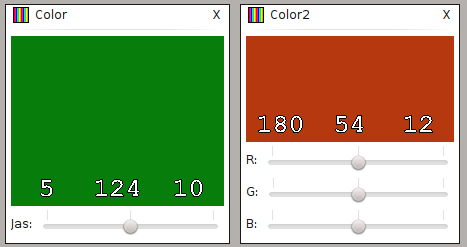
\includegraphics{img/w_col.png}
\caption{Widget: color}
\end{center}
\end{figure}
This widget shows incoming data as colored rectangle. Supported color formats:
\begin{itemize}
    \item {\bf RGB} (8b/channel, 3x uint8)
    \item {\bf RGB} (10b/channel, 3x uint16)
    \item {\bf RGB} (10b/channel, 1x uint32)
    \item {\bf Shades of gray} (8b/channel, 1x uint8)
    \item {\bf Shades of gray} (10b/channel, 1x uint16)
\end{itemize}
Widget supports brightness correction for all colors at once or for each color of RGB space separately.

\subsection{Widget: graph}
\begin{figure}[h]
\begin{center}
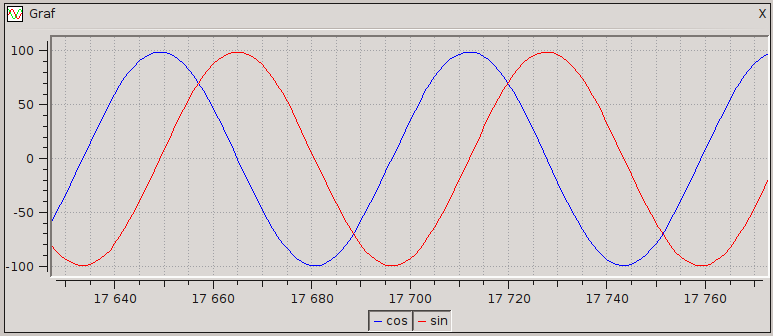
\includegraphics[scale=0.65]{img/w_graph.png}
\caption{Widget: graph}
\end{center}
\end{figure}
This widget shows data in graph -- order of the data is on the $x$ axis and data values on the $y$ axis. User can set name, color and data type of each graph curve and automatic scrolling, sample size and scale for graph. Graph also has legend which shows curve's names and colors, and curves can be hidden by clicking at their names in legend. Scale of each axis can be changed by scrolling the mouse wheel while hovering the cursor above axis. If the mouse is above graph area, mousewheel changes scale of both axes at once.
\begin{figure}[h]
\begin{center}
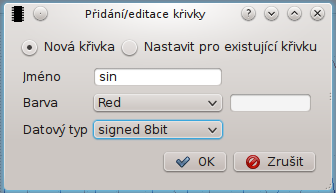
\includegraphics[scale=0.8]{img/w_graph_add.png}
\caption{Curve settings dialog}
\end{center}
\end{figure}

\subsection{Widget: script}
\begin{figure}[h]
\begin{center}
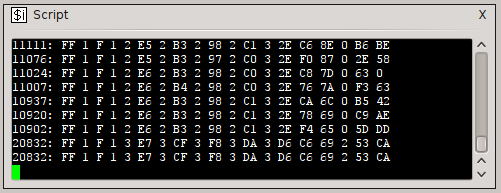
\includegraphics[scale=0.8]{img/w_script.png}
\caption{Widget: script}
\label{script_w}
\end{center}
\end{figure}
This widget uses user-written script to process data. Script can be written in Python or QtScript\cite{qtscript} (language based on ECMAScript\footnote{\It{ECMAScript} -- scripting language accoring to stadard ECMA-262 and ISO/IEC 16262}, same as JavaScript\footnote{\It{JavaScript} -- scripting languge used primarily on web}, which means JavaScript and QtScript are very similar).

Script can process incoming data, react to keypresses and send data to device. Basic output can be displayed in terminal (image \ref{script_w}), but it is also possible to use other widget types to show data (number, bar, ...).
%Script reference is in \hyperref[script_ref]{attachment A}.

Script editor has built-in code samples, for example how to set value of existing \It{number} widget, how to send data to device or how to react to keypresses (on image \ref{script_src} they are hidden under the lightbulb icon). Editor also has link to automatically generated documentation, which is available on \url{http://technika.junior.cz/docs/Lorris/}.

\begin{figure}[h]
\begin{center}
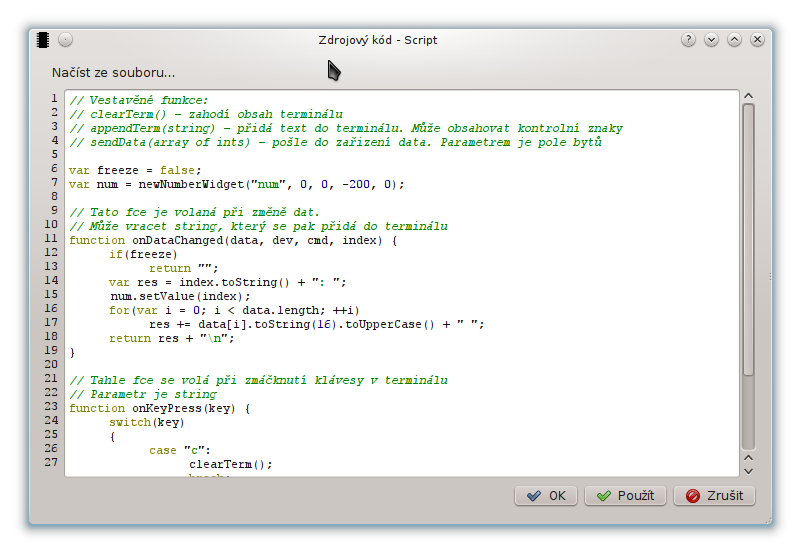
\includegraphics[width=\textwidth]{img/w_script_src.png}
\caption{Script editor}
\label{script_src}
\end{center}
\end{figure}

\subsection{Widget: circle}
\begin{figure}[H]
\begin{center}
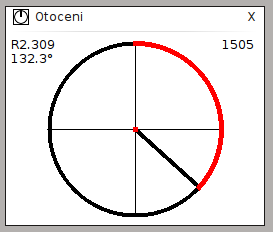
\includegraphics[scale=0.8]{img/w_circle.png}
\caption{Widget: circle}
\end{center}
\end{figure}
Widget \It{circle} shows incoming data as angle in circle, which is useful for example when displaying rotation of robot's wheel. Incoming data can be in degrees, radians or just number in certain range (eg. data from 12bit encoder in range from 0 to 4095).

\subsection{Widget: canvas}
\begin{figure}[H]
\begin{center}
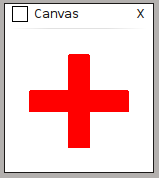
\includegraphics[scale=1]{img/w_canvas.png}
\caption{Widget: canvas}
\end{center}
\end{figure}
\It{Canvas} can be only controled from script and is supposed to be used to draw 2D graphics. It can draw lines, rectangles, circles and ellipses. Following code sample will draw red cross in the center of the widget.

\begin{listing}[H]
\begin{jscode}
Canvas.setLineColor("red");
Canvas.setFillColor("red");
// x, y, width, height
Canvas.drawRect(55, 10, 20, 110);
Canvas.drawRect(10, 55, 110, 20);
\end{jscode}
\caption{Drawing to canvas}
\end{listing}

\subsection{Widgets button and slider}
\begin{figure}[H]
\begin{center}
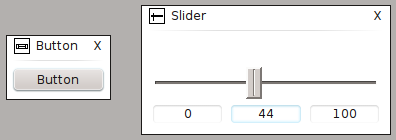
\includegraphics[scale=1]{img/w_btn_slider.png}
\caption{Widgets button and slider}
\end{center}
\end{figure}
These two widgets are used for interaction with script -- callback method in script is invoked on button click. In this method user can for example send a command to robot. Similarly, callback method is invoked after moving slider, so that user can for example change robot's movement speed. Keyboard shortcut can be assigned to button "click" action and for slider to gain focus, so that user can move it using arrow keys.
\begin{listing}[H]
\begin{jscode}
function Slider_valueChanged() {
    appendTerm("Slider value: " + Slider.getValue() + "\n");
}

function Button_clicked() {
    appendTerm("Button clicked\n");
}
\end{jscode}
\caption{\It{Slider} and \It{button} callbacks}
\end{listing}

\subsection{Widget: input}
\begin{figure}[H]
\begin{center}
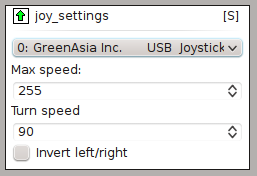
\includegraphics[scale=1]{img/w_input.png}
\caption{Joystick settings in widget \It{input}}
\label{input}
\end{center}
\end{figure}
This widget is also for interaction with script (user \It{input}), but script also defines interface itself -- the widget is empty by default and script has to create UI components, for example button or text field. This widget is a bit more complex, but it can create any of the UI components Qt Framework offers -- buttons, slider, text fields, combo boxes and so on. Code sample \ref{input_script} creates UI from image \ref{input}.

\begin{listing}[H]
\begin{jscode}
// args: Qt widget name, stretch value
var joyList = joy_settings.newWidget("QComboBox");
var maxSpdLabel = joy_settings.newWidget("QLabel", 1);
var maxSpd = joy_settings.newWidget("QSpinBox");
var turnSpdLabel = joy_settings.newWidget("QLabel", 1);
var turnSpd = joy_settings.newWidget("QSpinBox");
var invert = input.newWidget("QCheckBox");

// set QLabel text
maxSpdLabel.text = "Max speed:";
\end{jscode}
\caption{Adding UI components to widget \It{input}}
\label{input_script}
\end{listing}

\subsection{Widget: status}
\begin{figure}[H]
\begin{center}
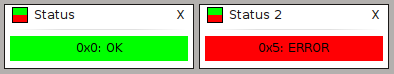
\includegraphics[scale=1]{img/w_status.png}
\caption{Widget status}
\end{center}
\end{figure}
\It{Status} is designed to show state of for example button (pressed/released) or error status from encoder (0 = okay, other values are error codes). User assigns states to incoming values (state consists of text and it's color, see image \ref{status_dlg}) and widget then shows active states. It supports "Unknown value", which is shown when incoming data don't match any defined status.
\begin{figure}[H]
\begin{center}
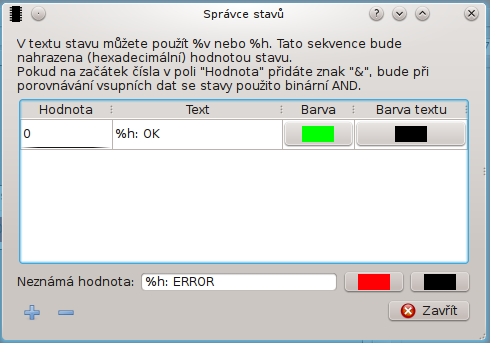
\includegraphics[scale=1]{img/w_status_dlg.png}
\caption{State definitions dialog}
\label{status_dlg}
\end{center}
\end{figure} 

\subsection{Widget: terminal}
\begin{figure}[H]
\begin{center}
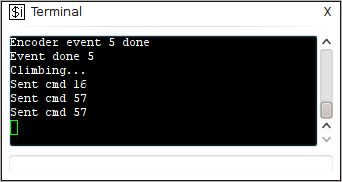
\includegraphics[scale=0.8]{img/w_terminal.png}
\caption{Widget terminal}
\end{center}
\end{figure}
This widget exists only for convenience of the user, it's widget \It{script} with preset code working exactly as terminal (sends keypresses, shows incoming data). User can edit predefined script, just like it was regular widget \It{script}.

\newpage
\setlength{\voffset}{0mm} % posune text/obrázek na této stránce, kam patøí
\pagestyle{plain}
\section{Module: Proxy between serial port and TCP socket}
\begin{figure}[H]
\begin{center}
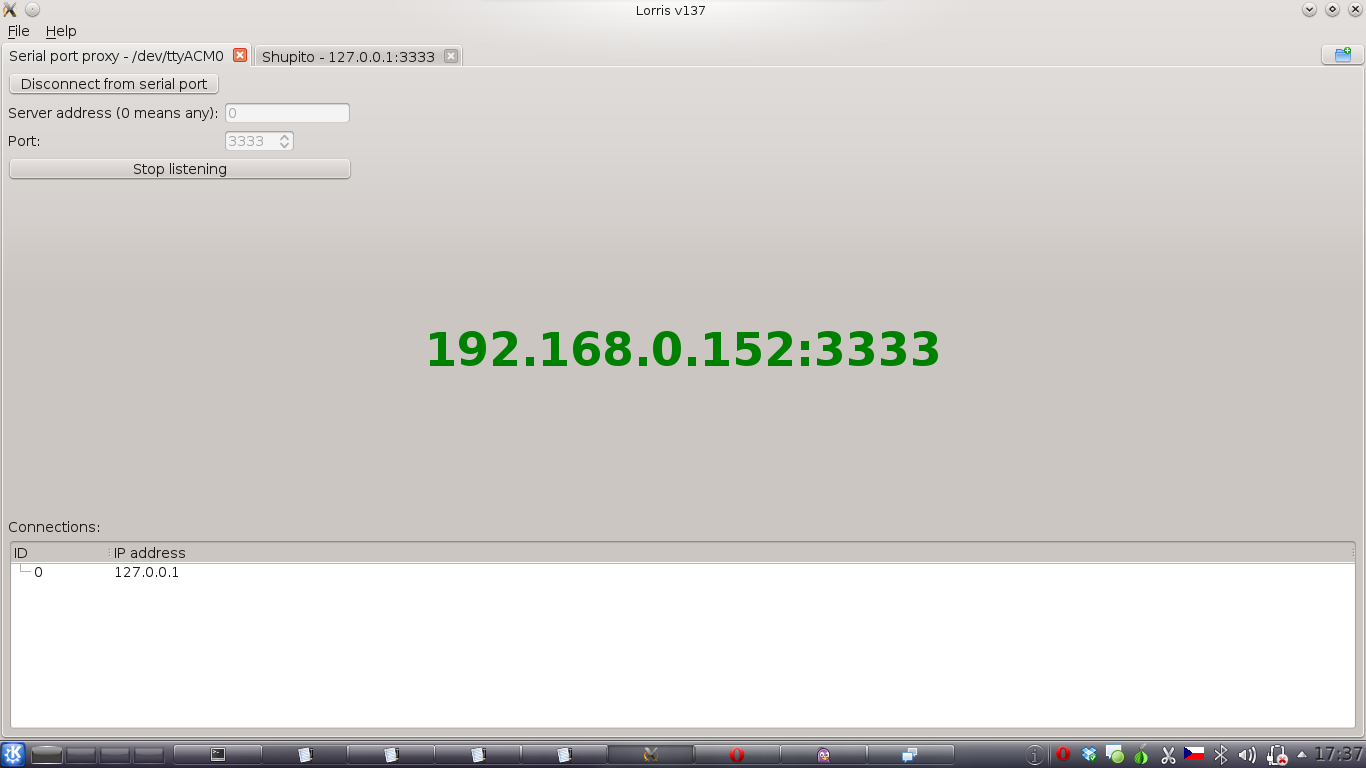
\includegraphics[width=\textwidth]{img/proxy.png}
\caption{Proxy between serial port and TCP socket}
\label{Shupito}
\end{center}
\end{figure}
Simple proxy which transfers data between serial port and TCP socket. It creates server the user can connect to from Lorris or other program on different computer. Data are transfered between serial port and connected clients.

\subsection{Proxy tunnel}
This module also adds new virtual connection -- "proxy tunnel". If another Lorris module uses this connection, it can send and receive data from all clients connected to proxy. This can be used to for example generate data in analyzer and then send them to multiple TCP clients.

\newpage
\setlength{\voffset}{0mm} % posune text/obrázek na této stránce, kam patøí
\pagestyle{plain}

\section{Module: programmer}
\begin{figure}[H]
\begin{center}
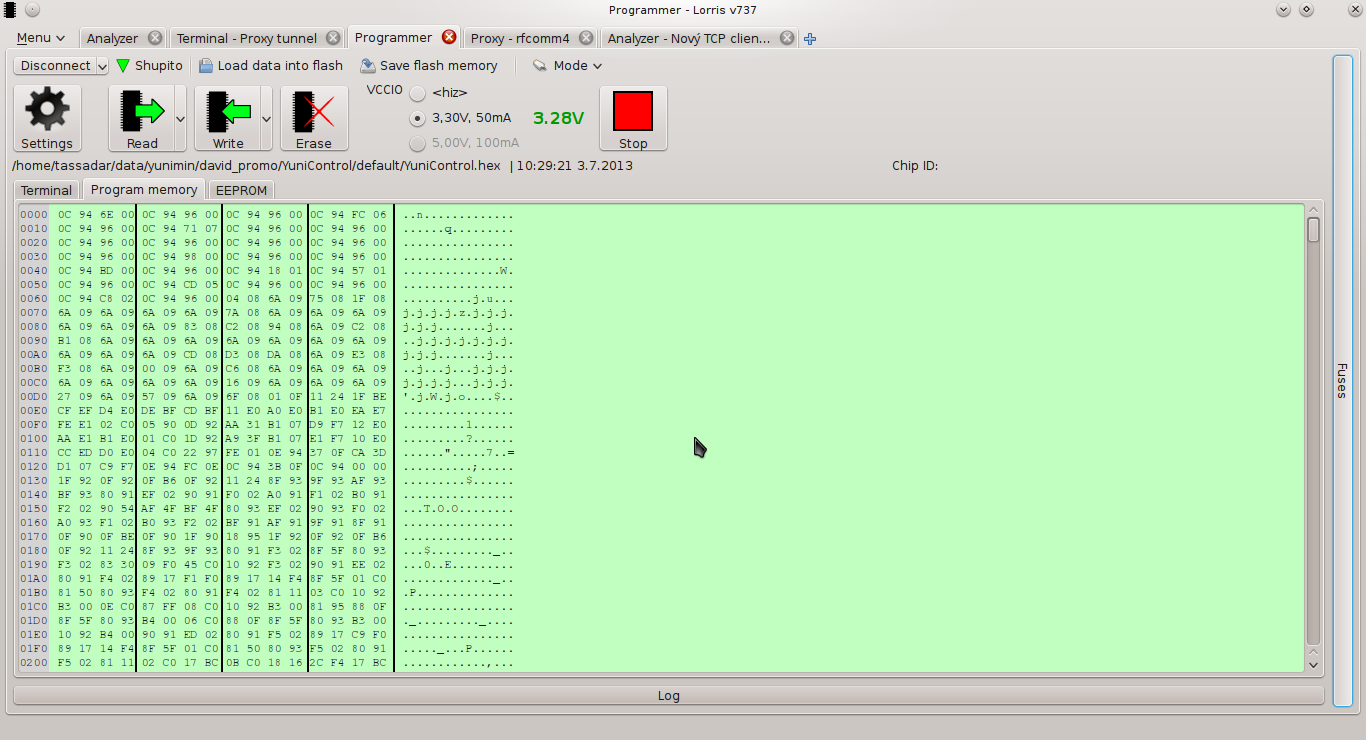
\includegraphics[width=\textwidth]{img/programmer.png}
\caption{Module programmer}
\label{prog_full}
\end{center}
\end{figure}

%TODO: rozšířit
This module acts as graphical interface for several types of programmers and bootloaders. The interface has two modes -- full (image \ref{prog_full}) and minimal (image \ref{prog_mini}). Full interface contains all buttons and settings for programming all memories of the chip, minimal interface contains only button which flashes main memory and button to stop chip. Minimal interface is convenient when using the split feature as demonstrated in image \ref{prog_mini}, because it uses only a small amount of space.

\begin{figure}[H]
\begin{center}
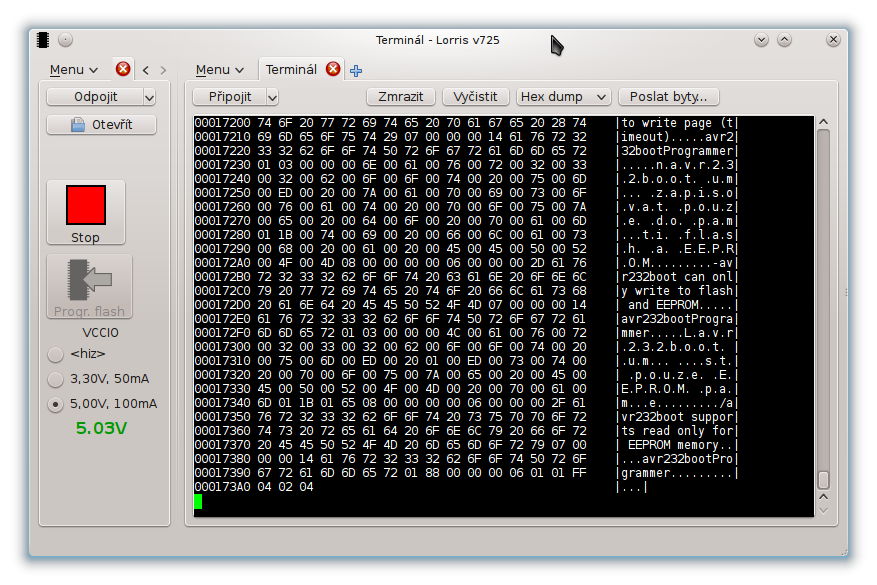
\includegraphics[width=\textwidth]{img/programmer_mini.png}
\caption{Minimal interface of module \It{programmer} (left) along with \It{terminal}}
\label{prog_mini}
\end{center}
\end{figure}

\subsection{Shupito programmer}
Shupito is microchip programmer created by Martin Vejnár. It can program microcontrollers using ISP\footnote{\It{In-system programming} -- interface which can programm chips directly on their PCB}, PDI\footnote{\It{Program and Debug Interface} -- interface by company Atmel with features similar to ISP} and JTAG\footnote{\It{Joint Test Action Group} -- interface standard IEEE 1149.1 which can be used to program and debug chips} interfaces.

Module programmer in Lorris is official interface for Shupito programmer. Most of Shupito communication is written by Martin Vejnár.

\subsubsection{UART tunnel}
\label{tunel}
Shupito can create tunnel\footnote{Direct connection between programmed chip and the computer via programmer} for UART interface from programmed chip to computer. Lorris can use this feature -- active tunnel creates new virtual connection and other modules can connect to it.

\subsection{Bootloader avr232boot}
Author of this bootloader is also Martin Vejnár. Avr232boot supports only Atmel ATmega chips and it is inspired by reference bootloader code for these chips, but it is designed to be as small as possible. Originally, it could only program flash memory of the chip (the one where program is stored), I added support for programming and reading of EEPROM\footnote{Flash memory which keeps data even without electricity. It is used to store for example program settings.} memory.

Lorris can use this bootloader to program flash memory and read and program EEPROM.

\subsection{Bootloader AVROSP}
\It{AVR Open Source Programmer} is protocol used by several bootloaders by Atmel for chips ATmega and ATxmega. Lorris can use this protocol to program and read both flash and EEPROM memory of the chip.

\newpage
\section{Module: terminal}
\begin{figure}[H]
\begin{center}
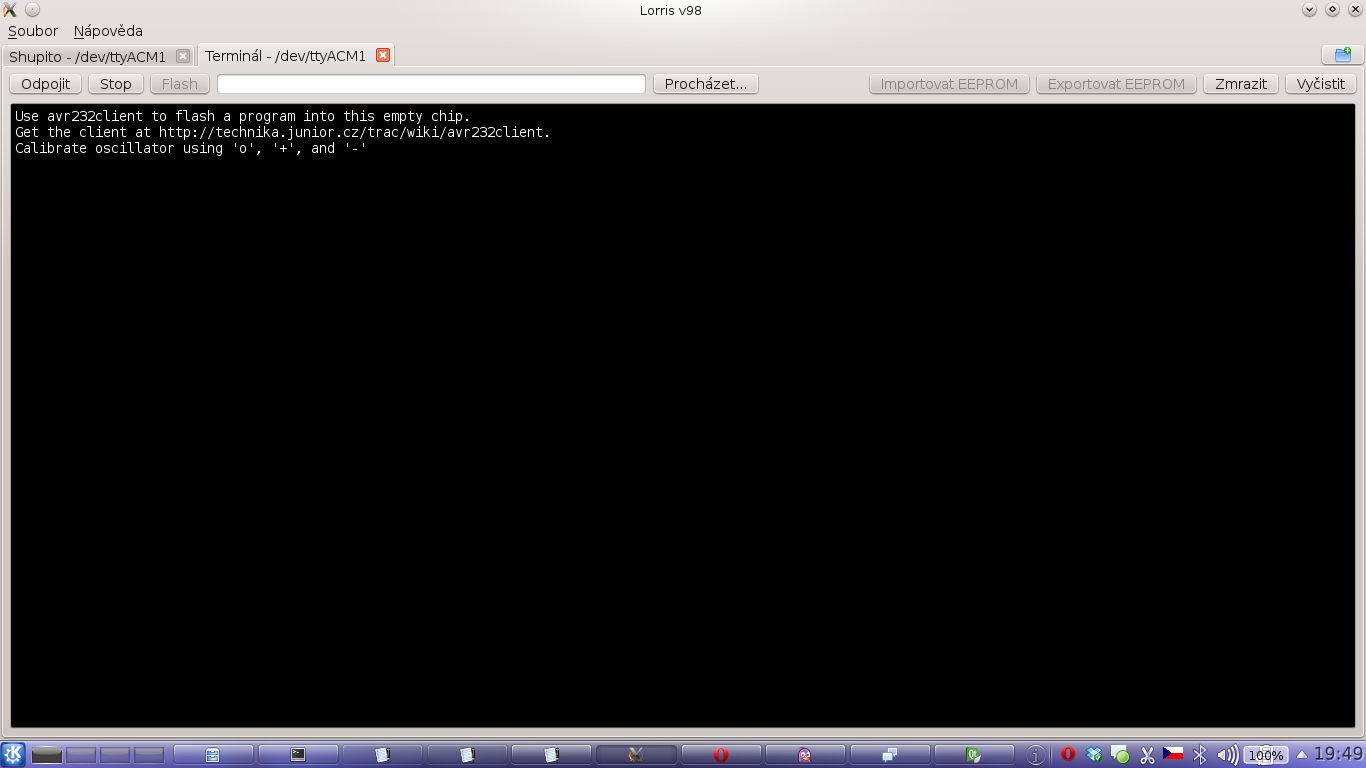
\includegraphics[width=\textwidth]{img/terminal.png}
\caption{Module terminal}
\label{Terminal}
\end{center}
\end{figure}
Fundamental tool for every developer, classic text terminal. It shows incoming data in either text mode or as hexadecimal values of each byte and sends keypresses.

User can set terminal's colors, font size, which sequence of control characters should be sent after return key press and behavior of several control characters (for example if character \verb|\n| should create new line or not).

\newpage
\section{Joystick support}
Lorris supports joystick in module analyzer to for example control robot. At first, I've used SDL\cite{sdl} library to access joystick, but it was not really suitable for my use -- SDL is video game library, joystick support is only one of many subsystems this library contains. It's architecture also wasn't ideal to use in Lorris.

I haven't found any suitable replacement of SDL, so I wrote my own library.

It is called {\bf libenjoy}, it works under Windows and Linux and it is very small and simple. One major advantage over SDL is that it can remember connected joysticks -- if you disconnect joystick and then plug it in again (because you want to reorganize cables on your desktop or because of bad USB connection), it will open the joystick again by itself -- without any user interaction.

Libenjoy is released under GNU LGPLv2.1\cite{lgpl} license.
\begin{itemize}
\item GIT repository: \url{https://github.com/Tasssadar/libenjoy}
\end{itemize}

\newpage
\section{Usage examples}
\subsection{Color sensor testing}
{\bf Situation:} I'm builing robot for some competition (Eurobot, RobotChallange, ...) and I want to use color sensor to direct the robot. I also want to test the color sensor, so I've made simple circuit with chip and color sensor. Chip will instruct the sensor to measure the colors and send color values to computer via UART interface.\\
\\
\noindent{\bf Solution:} I use Shupito to program the chip and it's shupito tunnel to read data from UART interface. I connect analyzer module to shupito tunnel and then use widget \It{color} to show me color measured by the sensor.

\begin{figure}[h]
\begin{center}
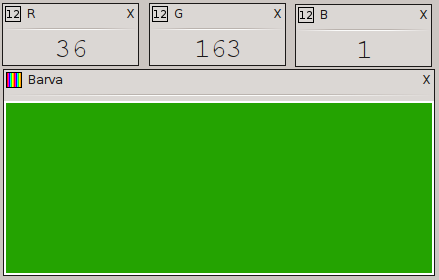
\includegraphics{img/use_color.png}
\caption{Color in analyzer module}
\end{center}
\end{figure}

\newpage
\subsection{Encoder testing}
My schoolmate Marek Ortcikr made SOČ named \It{Modular building blocks for robots} (\It{Modulární stavba robota}). One of the blocks was magnetic encoder. This encoder looks like another wheel for the robot, but little magnet is placed in wheel's axis. Encoder chip placed directly in front of the magnet detects orientation of magnetic field generated by the magnet and therefore rotation of the wheel itself.

Encoder is able to calculate distance covered by the robot and it's speed and acceleration by monitoring changes in wheel's rotation.

\begin{figure}[H]
\begin{center}
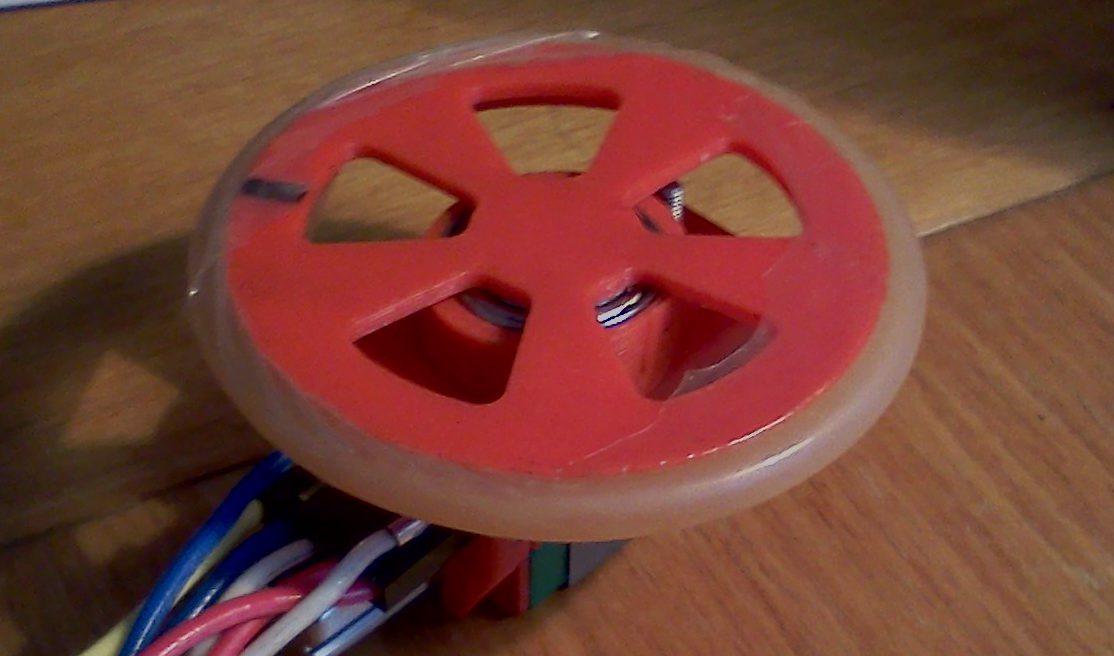
\includegraphics[width=\textwidth]{img/enc_real.png}
\caption{Magnetic encoder}
\end{center}
\end{figure}

Lorris was used to demonsrate encoder's function on national tier of SOČ competition. Whole interface can be seen on image \ref{analyzer_all} on page \pageref{analyzer_all}, following text addresses each part individually.

\begin{figure}[H]
\begin{center}
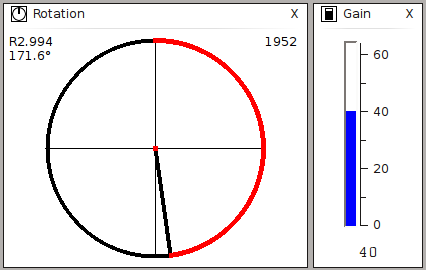
\includegraphics[width=\textwidth-45pt]{img/enc_circle.png}
\caption{Rotation of the wheel}
\end{center}
\end{figure}
Widget \It{circle} is used to represent current rotation of encoder's wheel. Current value read from encoder (0 to 4095) is placed in top right corner, number in left corner are values converted to radians and degrees.

Values in widget \It{bar} named "Gain" represent strength of the magnetic field, thus how far is the magnet from the encoder's chip. Value is in range from 0 to 63, ideal is about the middle of this range.

\begin{figure}[H]
\begin{center}
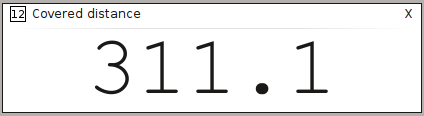
\includegraphics[scale=0.85]{img/enc_dist.png}
\caption{Covered distance}
\end{center}
\end{figure}
This is widget \It{number} displaying covered distance in millimeters. Encoder sends this value in $\frac{1}{4096}$ of wheel's circumference, so formula \verb|%n/32.5949| has to be used to convert it to millimeters.

\begin{figure}[H]
\begin{center}
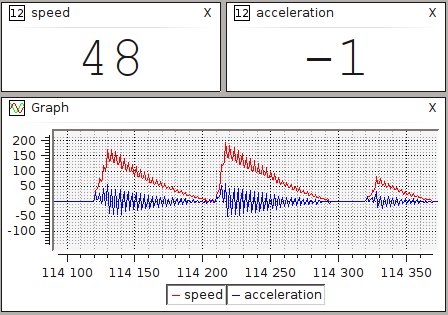
\includegraphics[width=\textwidth-60pt]{img/enc_spd.png}
\caption{Speed and acceleration}
\end{center}
\end{figure}
Current speed and accelertaion are displayed in two widgets \It{number}, and widget \It{graph} underneath shows speed as red curve and acceleration as the blue one.

\begin{figure}[H]
\begin{center}
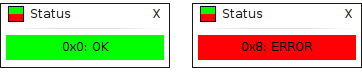
\includegraphics[width=\textwidth]{img/enc_status.png}
\caption{Encoder's status}
\end{center}
\end{figure}
Encoder's chip also sends status informations. If everything is okay, it sends number \verb|0x0|, if some problem is encountered, it returns one of the error codes (e.g. \verb|0x8| means that there is no magnet present). Widget \It{status} shows current error code and color according to informations from encoder.

\begin{figure}[H]
\begin{center}
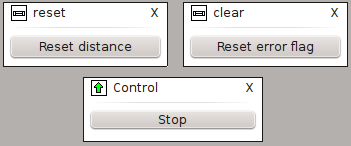
\includegraphics[width=\textwidth-50pt]{img/enc_ctrl.png}
\caption{Encoder's controls}
\end{center}
\end{figure}
These \It{button} and \It{input} widgets are here to be used to control the encoder. Button "reset" resets distance counter to zero, button "clear" sends command to clear error code (it still stays even if cause of the error was fixed, it has to be manually cleared) and button "Control" starts/stops data stream from the encoder. All of these widgets are connected to script (image \ref{analyzer_all} does not contain \It{script} widget because it didn't fit the window) which reacts to button clicks by sending appropriate commands to encoder.

\begin{listing}[H]
\begin{jscode}
var run = true;
function reset_clicked() {
    sendData(new Array(0xFF, 0x01, 0x01, 0x00));
}
function clear_clicked() {
    sendData(new Array(0xFF, 0x01, 0x01, 0x01));
}
function startStop_clicked() {
    run = !run;
    startStopBtn.text = run ? "Stop" : "Start";
    sendData(new Array(0xFF, 0x01, 0x02, 0x02, run ? 1 : 0));
}
\end{jscode}
\caption{This script sends commands to encoder}
\end{listing}

\newpage
\subsection{Tuning of PID regulator}
{\bf Situation:} Robot can't go straight because each motor has slightly different speed. I decided to solve this problem using PID regulator. But PID regulator needs several constants to be correctly set. \\
\\
{\bf Solution:} Robot's program is sending current motor speed and PID constants values to computer and also allows changing those constants via UART interface. This program is flashed into robot over bluetooth using avr232boot bootloader -- I don't have to use any programmer, which would require cable connection.

I use widgets \It{number} and \It{graph} to show current PID constants and speed of both motors. Then I write simple script which will change PID constants after keypress and starts/stops robot.

I've used this process to tune PID regulator on my 3pi\cite{3pi} robot. I've attened to \It{Line Follower Standard} competition on Robotic Day 2012 in Prague\cite{rob_den} with this robot and I've won the second place from total of 22 robots.

\begin{figure}[H]
\begin{center}
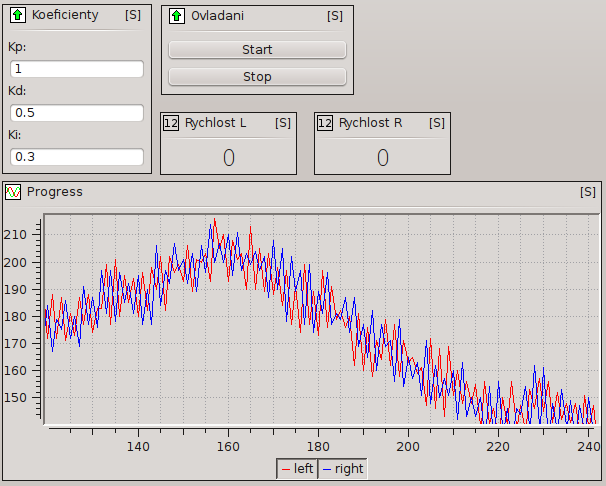
\includegraphics[scale=0.55]{img/use_pid.png}
\caption{PID regulator tuning}
\end{center}
\end{figure}

\newpage
\subsection{Developement of robot for Eurobot 2011 competition}
Usage of my Lorris program is exaplained here using example case of robot, which was developed on our school (SPŠ a VOŠ technická, Sokolská~1, Brno) in 2011 to compete in Eurobot contest.

Goal and game mechanics are different each year, in 2011 the goal was to play something like simplyfied chess game. Game fields was divided to red and blue squares and upon it were "pawns" (yellow discs) and robots had to move the pawns to squares of their color or make "towers" by putting pawns top of each other. Winner was the robot with the most points, which were awared for each pawn on square of robot's color and for built towers. In addition to that, robot's had to detect each other in order not to collide (e.g. using ultrasound range finders). For complete rules, results and more informations, see the web page of Eurobot 2011\cite{eurobot11}.

Most pressing need for tool, which would let us test and debug all of the robot's functions and components quickly and easily, has arisen. Mainly usage of the Analyzer tool is presented here, due to the fact that it is the most visible part of the program. Other tools (Programmer, Terminal) were also used, for example for writing program into the robot's chip.

This example contains simple user interface for controling, testing and debugging of our robot, but this interface can also be used for other robots. You can also create new interface to fulfill your needs, for example when the robot is too atypic and requires different type of controls.

\newpage
\subsubsection{Robot's frame}
Body of the robot  was constructed first and even in this early stage, my Lorris program was already used. We needed to test if all the motors and servos work properly and how exactly they behave, so I assembled a small group of widgets in Lorris, which would allows to control the robot via joystick. Several widgets were used, namely \Iv{Script}, which was reading data from joystick, calculating the speed values for motors and sending them to the robot. Next, widget \It{Input}, which contained settings joystick parameters and lastly, 2 widgets \It{number} with motors̈́' speeds.
\vspace{30mm}
\begin{center}
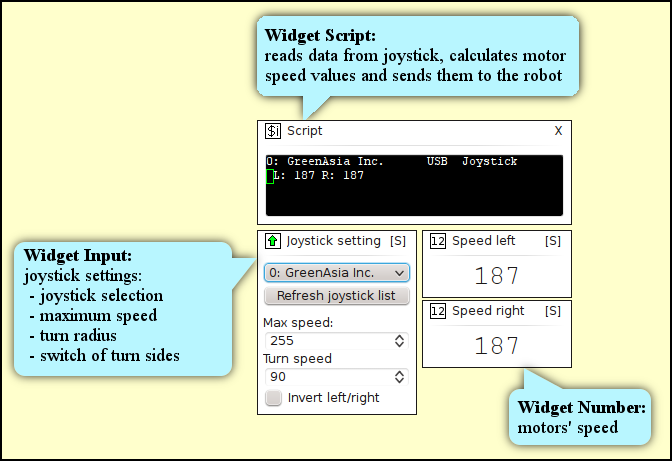
\includegraphics[width=\textwidth]{img/joystick_david.png}
\end{center}

\newpage
\subsubsection{Debugging and adjusting of sensors}
When the mechanical frame was complete and tested, all sensors were added to the robot. After that, interface to actually see sensor values was needed, so I created interface for this purpose in Analyzer. It uses mainly \It{script}, \It{number} \It{color} and \It{status} widgets. Each and every one of these widgets can be moved around Analyzer's worspace and resized. That makes it possible to place widgets so that their positions coresponds with their real positions on the robot. Top view appears to be ideal for this task.
\vspace{10mm}
\begin{center}
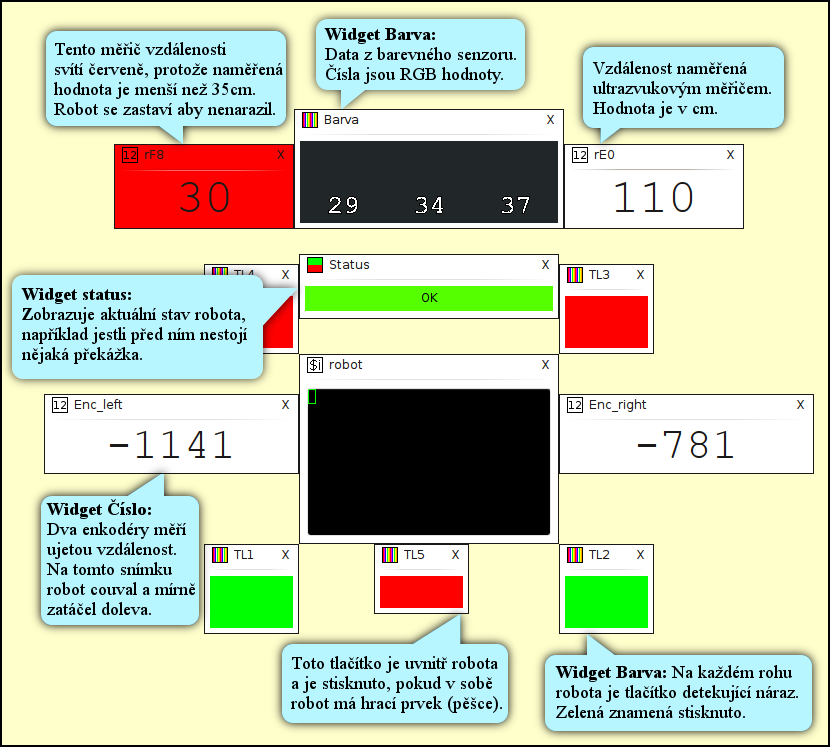
\includegraphics[width=\textwidth]{img/sensors_david.png}
\end{center}

\newpage
\subsubsection{Programming of robot's reactive behavior}
Peak of the developement was programming of its behavior on the game field. For this occasion, widget \It{script} in my Lorris program was used to large extent. Scripting enviroment which encapsulated robot's basic command sets was created in this widget. These command sets allows us to create more complicated behavioral patterns for the robot. It would be possible to write script for the robot directly, but this enviroment considerably simplified and sped up the developement. Another fact is also worth noticing -- widget \It{Script} was used here not only to control the robot, but also to improve functionality of the Analyzer tool itself.

In this example, I use simple "actions", which are executed by the robot step by step. Each action has 3 main parameters -- direction of movement, when the robot should stop and what should it do when it arrives at it's target destination. Each action can be changed directly in the scripting enviroment, bypassing the need to re-program robot after every change. All other parts of Lorris are still working, even when the robot is controlled by the script. That makes it possible to keep track of robot's state as well as all his sensors and quickly find the source of possible unexpected behavior.
\\
\\
\noindent\It{You can find image no. \ref{david_ctrl} which belongs to this part of the text in attachments on page \pageref{david_ctrl}.}

\newpage
\section{Android application}
\begin{figure}[H]
\begin{center}
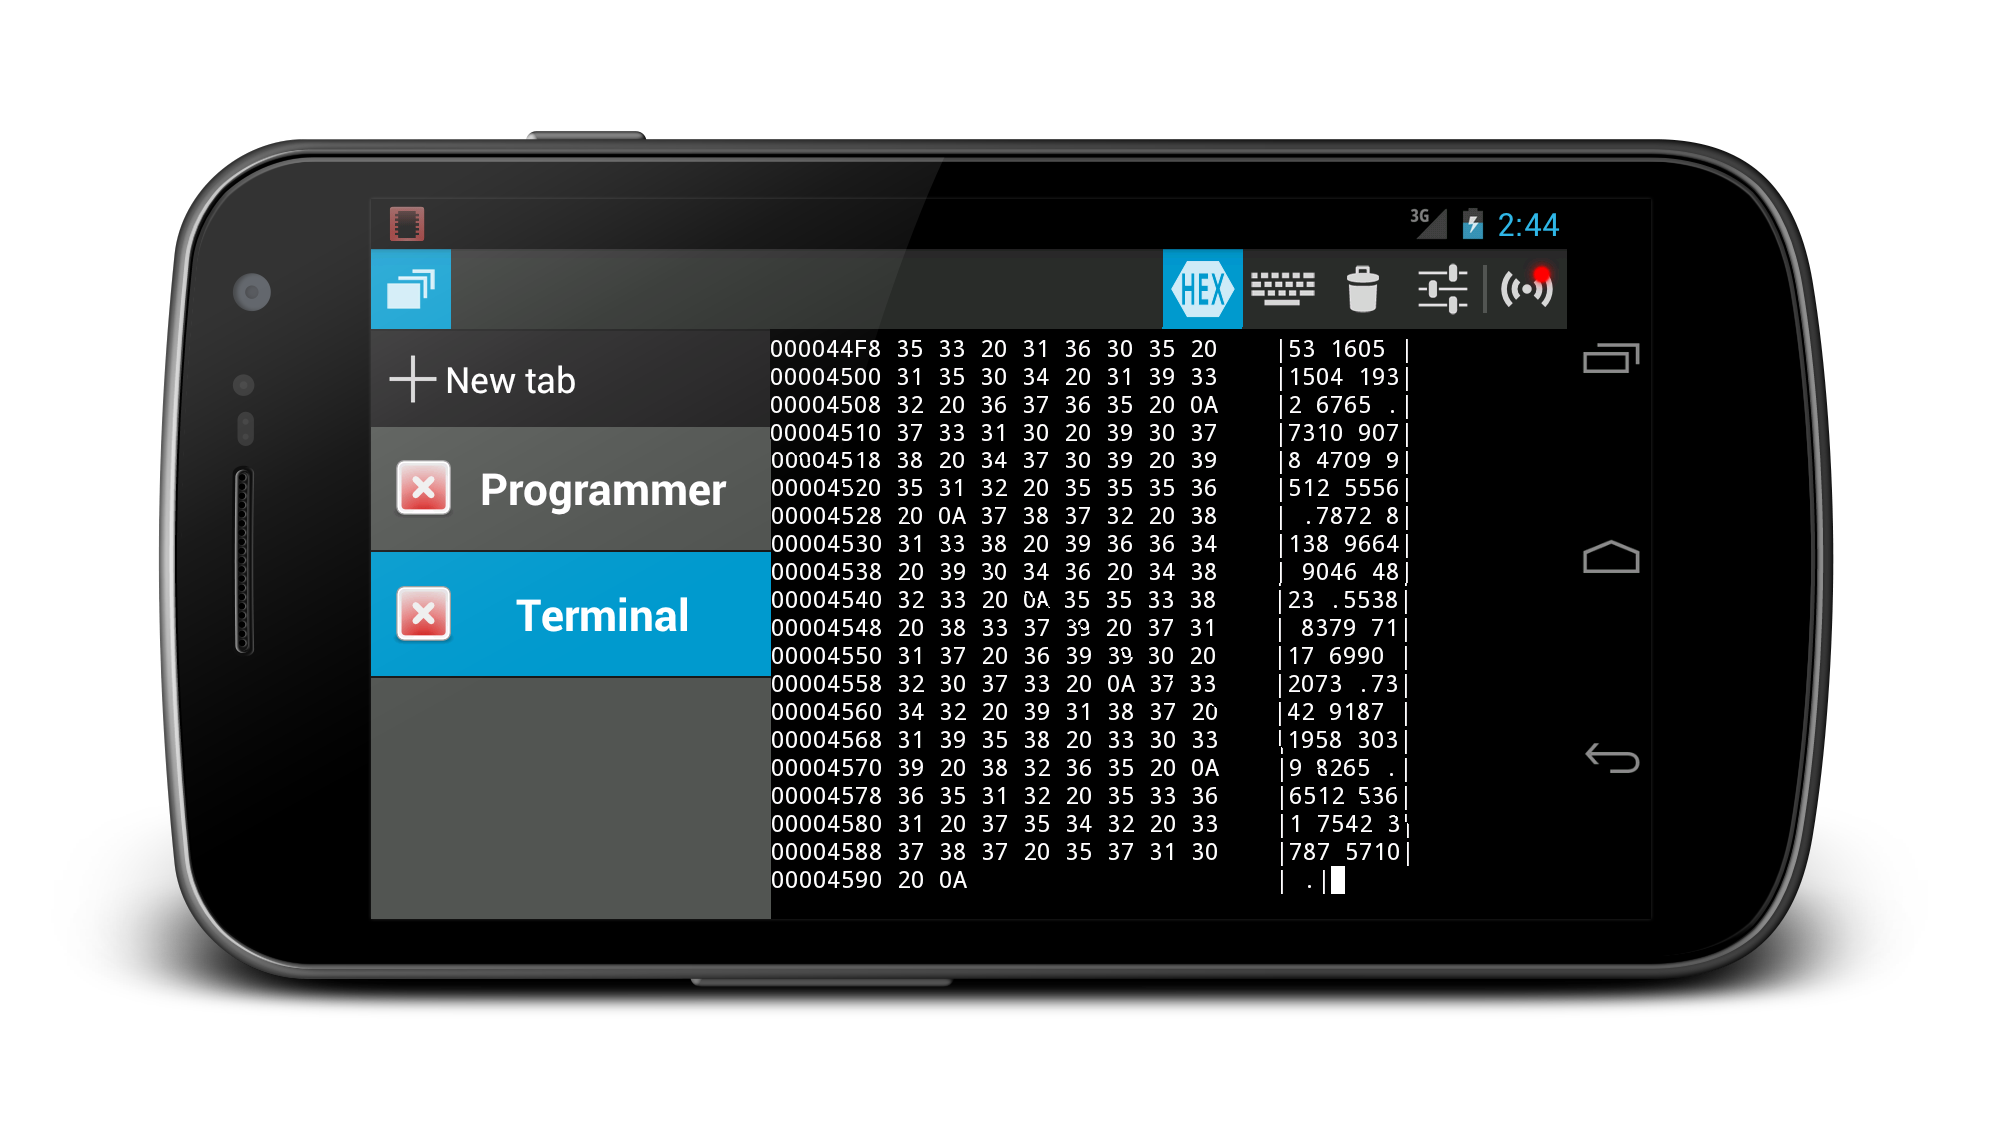
\includegraphics[width=\textwidth]{img/mobile.png}
\caption{Lorris mobile}
\end{center}
\end{figure}

Application for Google Android\cite{android} platform is the next step in Lorris' developement, because mobile devices with this operating systems are almost always at hand and are sufficient to quickly solve smaller problems.

Application {\bf Lorris mobile} acts as portable addition to desktop version of Lorris -- it may not have all the features of desktop version, but helps when you need to quickly correct or debug something out in the field.

App works on all tablets and phones with Android OS version 2.2 and higher, it is optimized also for bigger tablet screens and can be obtained in official distribution channel of Android application -- in Google Play Store\cite{gplay}. You can find it by searching for "Lorris".

Lorris mobile has similiar architecture as desktop Lorris. User has to create session first, so that everything he opens can be saved (image \ref{mobile_session}). After user loads the sessions, he gets to main screen of the application, where he can open modules in tabs, much like in desktop Lorris (image \ref{mobile_tabs}).

\begin{figure}[H]
\begin{center}
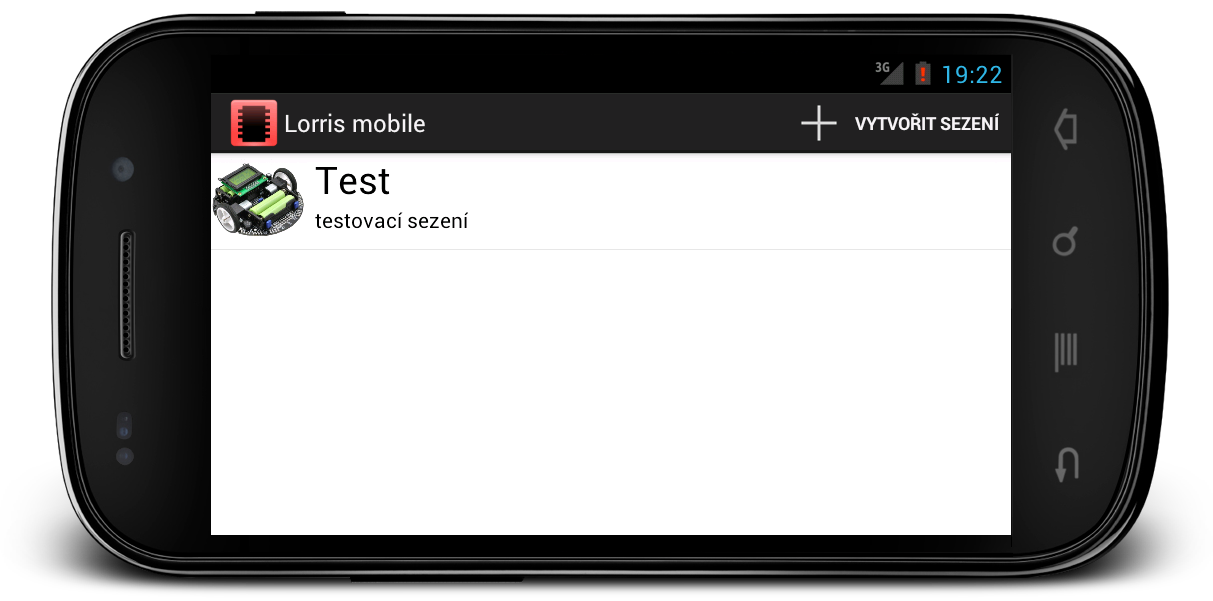
\includegraphics[width=\textwidth]{img/mobile_session.png}
\caption{Lorris mobile -- session selection}
\label{mobile_session}
\end{center}
\end{figure}
\begin{figure}[H]
\begin{center}
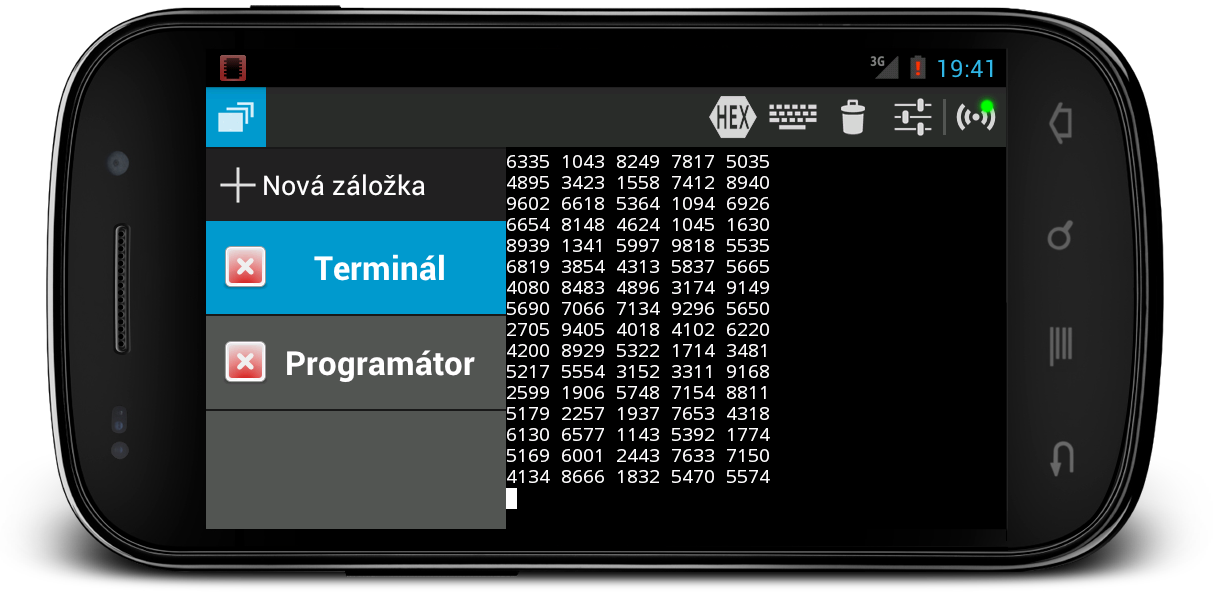
\includegraphics[width=\textwidth]{img/mobile_tabs.png}
\caption{Lorris mobile -- switching tabs}
\label{mobile_tabs}
\end{center}
\end{figure}

\subsection{Programmer}
\begin{figure}[H]
\begin{center}
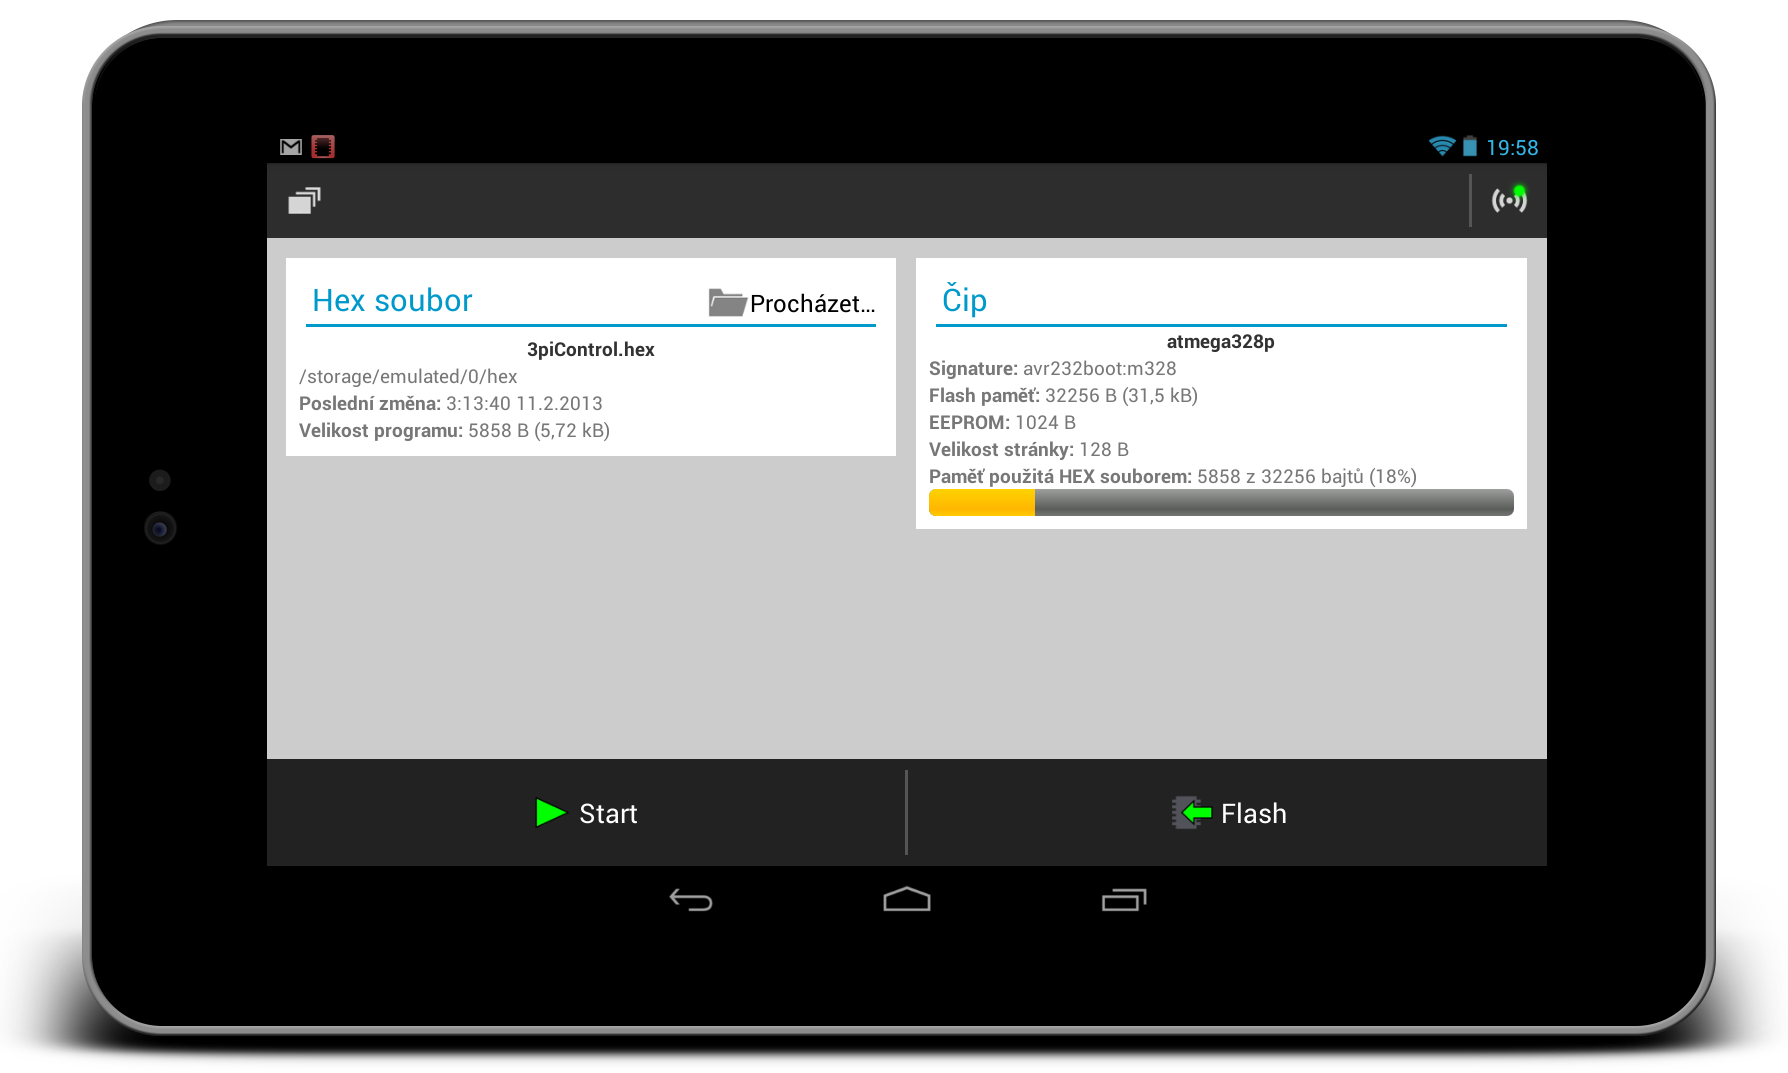
\includegraphics[width=\textwidth]{img/mobile_programmer.png}
\caption{Lorris mobile -- programmer}
\end{center}
\end{figure}
Module programmer can program chips using bootloaders {\bf avr232boot} and {\bf AVROSP} and also using Shupito programmer, if the device has USB host capabilities.

This part of Lorris mobile uses pieces of native code from desktop Lorris, which means the code is faster and easier to maintain.

\subsection{Terminal}
\begin{figure}[H]
\begin{center}
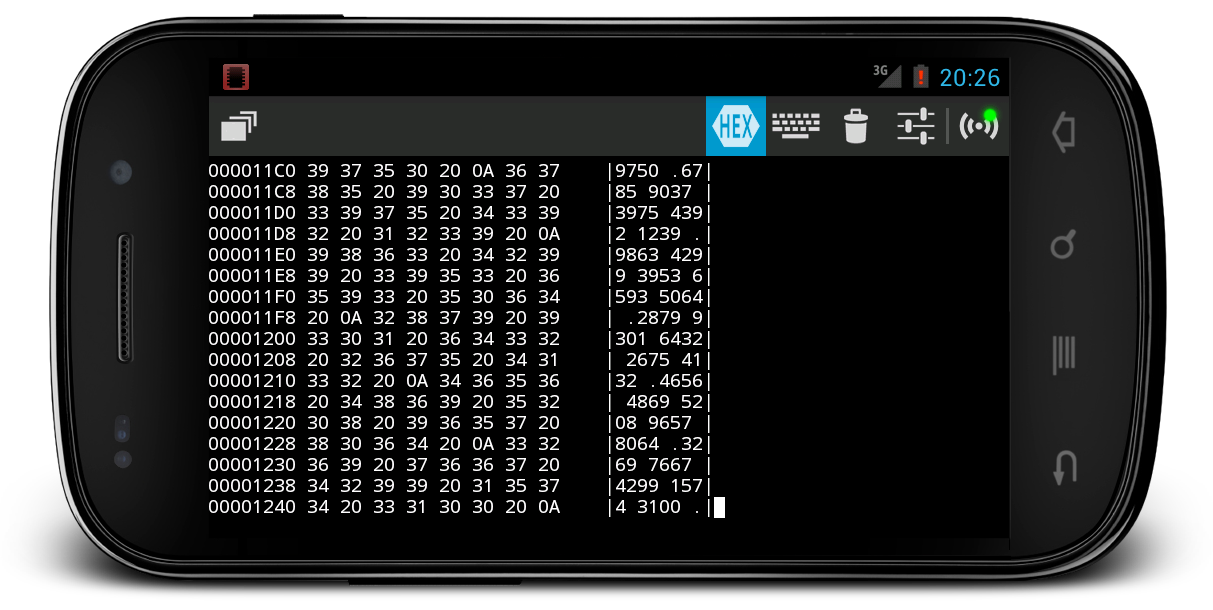
\includegraphics[width=\textwidth]{img/mobile_term.png}
\caption{Lorris mobile -- terminal}
\end{center}
\end{figure}
Classic terminal. Is has most features of the terminal in desktop version -- it displays data (as text or hexadecimal values), sends keypresses and user can set terminal's colors, font size and which control characters are sent after return key press.

\newpage
\section{Real world usage}
\label{usage}
Members of some of the technical clubs on DDM\footnote{\It{Dům dětí a mládeže} -- Organization which does clubs, camps or trips for kids} Junior\cite{junior} in Brno became the first users of Lorris toolbox on the very beginning of its development several years ago. Lorris helps there with developement of various devices, mainly robots, and kids who learn how to program microchips use \It{Shupito} programmer and thus also the Programmer module in Lorris. Modules terminal and analyzer are also useful during microchip programming lessons, terminal for simple communication with the chip and later analyzer for more advanced data processing.

Lorris is ideal for use in DDM Junior also because it is free -- bigger company which makes microchip applications would probably get expensive commercial program similar to Lorris or develop its own single-purpose applications. However, solution used by large companies is somewhat unaccessible for state-funded institutions.

Nowaday Lorris has about 20 users on DDM Junior alone. Number of users however rising thanks to gradual spreading of \It{Shupito} programmer among users in whole Czech Republic.

\vspace{10mm}

\noindent I use Lorris whenever I work with robots and/or microcontrollers -- to display data, program chips or control whole devices. Following list presents only some of the most significant applications made by other Lorris users:
\begin{itemize}
    \item Development of several robots for this year's Robotic day\cite{rob_den_new}
    \item Programming of widge variety of microchips, using either \It{Shupito} programmer or bootloaders
    \item Development of \It{Shupito} itself
    \item Development of cheap logic probe
    \item Debugging of chips for control of three-phase motors (i.e. \It{drivers})
    \item Developmnet of system for controlling of up to 128 RGB LEDs for illumination of model plane
    \item Construction and programming of digital radio transmitter with ARM processor (semestral work)
    \item Developmnet of line following robot (graduation work)
    \item Tuning of PID controller
\end{itemize}

%\newpage
\section*{Conclusion}
\addcontentsline{toc}{section}{Conclusion}
After several years of developement, I can certainly say the application meets all the requirements declared in chapter \ref{motivace}:
\begin{enumerate}[label=\Has\hspace{1.5mm}\arabic{*}.]
    \item Ability to process data from device and show them clearly % 1
    \item Support for many formats of incoming data% 2
    \item Quick and simple to use% 3
    \item Support for other operating systems than MS Windows % 4
    \item Low price% 5
    \item Ability to easily expand program, ideally open-source % 6
    \item No dependencies on other applications (eg. MS Office Excel) % 7
\end{enumerate}
On top of that, the program greatly outdoes original goals -- it can also send data to device, program microchips and create proxy between serial port and TCP socket. In comparison to other applications I've found (as described in introduction) Lorris is also the only one which allows user to write his own script to parse data.

Lorris has already been used in several real-world applications and it also has growing ranks of satisfied users, as described in chapter \ref{usage}.

The application is continuously being enhaced, it is possible to virtually indefinitelly add either more widgets to Analyzer (compass, gauge meter, ...) or whole new modules (e.g. interface for cheap logic probe currently in developmet by Martin Vejnár). The program consist from about 32 thousand lines of code (without thir-party libraries) at this time (3.4.2013).

Enclosed CD contains source code, orientation video and promotional poster.
\begin{figure}[H]
\begin{center}
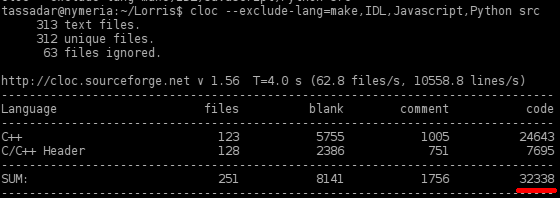
\includegraphics[width=\textwidth]{img/cloc_edit.png}
\caption{Lines of code counted by program CLOC\cite{cloc}}
\end{center}
\end{figure}

In the future, I would like to continue in adding new features to both computer and Android version of Lorris and in increasing of awarness about this useful piece of software.

%%%%%%%%%%%%%%%%%%%%%%%%%%%%%%%%%%%%%%%%%%%%%%%%%%%%%%%%%%%%%%%%%%%%%%%%%%%



\newpage
\section*{ATTACHMENT A:}
\section*{Third-party libraries}
\addcontentsline{toc}{section}{ATTACHMENT A: Third-party libraries}
\begin{itemize}
    \item {\bf Qwt}\cite{qwt} is library for Qt Framework which contains several widgets for techical applications -- graphs, bars, compasses, gauge meters or similar. 
    \item {\bf QExtSerialPort}\cite{qext} provides connection to serial port and also enumerates serial ports found in the computer.
    \item {\bf QHexEdit2}\cite{qhex} is hex editor used to show content of chip's memory in module Programmer. I changed few mostly visual details in this library.
    \item {\bf Tango Icon Library}\cite{tango} is set of icons released to the Public Doamain. Icons from this set on many places throughout the application.
    \item {\bf EcWin7}\cite{ecwin7} is library which provides API for progressbar built into task bar items in Windows 7.
    \item {\bf QScintilla2}\cite{qsci} is advanced text editor for Qt
    \item {\bf PythonQt}\cite{pythonqt} -- python bindings for Qt.
    \item {\bf Python}\cite{python} is programming language, Lorris uses several parts of it's interpreter in combination with Python Qt.
    \item {\bf Qt Solutions}\cite{qtsolutions} is collection of several addon classes for Qt.
    \item {\bf libyb}\cite{libyb} is library which provides communication with the \It{Shuputo} programmer
\end{itemize}

\section*{ATTACHMENT B:}
\section*{Licenses}
\addcontentsline{toc}{section}{ATTACHMENT B: Licenses}
Lorris is released under the GNU GPLv3\cite{gpl3}, licenses of used applications and libraries are as follows:
\begin{itemize}
    \item {\bf Qt Framework} is released under GNU LGPLv2.1\cite{lgpl}
    \item {\bf Qwt} is distrubuted under the Qwt license\cite{qwtlicense}, which is based of GNU LGPLv2.1
    \item {\bf QExtSerialPort} is released under The New BSD License\cite{newbsd}
    \item {\bf QHexEdit2} is released under the GNU LGPLv2.1
    \item {\bf Tanto Icon Library}\cite{tango} is released to the Public Domain
    \item {\bf EcWin7} is released under the GNU GPLv2
    \item {\bf QScintilla2} is released under the GNU GPL v2 a~v3
    \item {\bf libenjoy}\cite{libenjoy} is released under the  GNU LGPLv2.1
    \item {\bf PythonQt} is released under the GNU LGPLv2.1
    \item {\bf Python} is released under the PSF License agreement\cite{psf}
    \item {\bf Qt Solutions} is distrubuted under The New BSD License
    \item {\bf libyb} is released under the Boost Software License\cite{boost}
\end{itemize}

All of these licenses allow free usage and spreading of the code.

\newpage
 \section*{ATTACHMENT C:}
 \begin{thebibliography}{99}
\addcontentsline{toc}{section}{ATTACHMENT C: References}
 %% 99 znamená, že maximální délka čísla literatury jsou dva znaky
% seznam samozřejmě změníte podle svého, tohle je pouze ukázka formátování

    \bibitem{serialchart} \It{SerialChart} -- Analyse and chart serial data from RS-232 COM ports \\
    \url{http://code.google.com/p/serialchart/}\\
    (Prior to 2.\,25.\,2013)

    \bibitem{winwedge} \It{WinWedge} -- RS232 data collection software \\
    \url{http://www.taltech.com/products/winwedge/}\\
    (Prior to 2.\,25.\,2013)

    \bibitem{serialdatalogger} \It{Advanced Serial Data Logger} \\
    \url{http://www.aggsoft.com/serial-data-logger.htm}\\
    (Prior to 2.\,25.\,2013)

    \bibitem{stamplot} \It{StampPlot Pro} -- Graphical Data Acquisition and Control \\
    \url{http://www.selmaware.com/stampplot/index.htm}\\
    (Prior to 2.\,25.\,2013)

    \bibitem{labview} \It{LabVIEW} -- Laboratory Virtual Instrumentation Engineering Workbench \\
    \url{http://sine.ni.com/np/app/main/p/docid/nav-104/lang/cs/}\\
    (Prior to 3.\,6.\,2013)

    \bibitem{qtfrm} \It{Qt} -- Cross--platform application and UI framework \\
    \url{http://qt-project.org/}\\
    (Prior to 2.\,25.\,2013)

    \bibitem{debian} \It{Debian Linux} -- The Universal Operating System \\
    \url{http://www.debian.org/}\\
    (Prior to 2.\,25.\,2013)

    \bibitem{github} \It{GitHub} -- Social Coding \\
    \url{https://github.com}\\
    (Prior to 2.\,25.\,2013)

    \bibitem{qtscript} \It{Making Applications Scriptable} \\
    \url{http://qt-project.org/doc/qt-4.8/scripting.html}\\
    (Prior to 2.\,25.\,2013)

    \bibitem{xboot} \It{XBoot} -- Extensible bootloader for ATMEL XMEGA microcontrollers \\
    \url{http://code.google.com/p/avr-xboot/}\\
    (Prior to 3.\,6.\,2013)

    \bibitem{sdl} \It{SDL} -- Simple Directmedia Layer \\
    \url{http://www.libsdl.org/}\\
    (Prior to 2.\,13.\,2013)

    \bibitem{3pi} \It{Pololu 3pi Robot} \\
    \url{http://www.pololu.com/catalog/product/975}\\
    (Prior to 2.\,25.\,2013)

    \bibitem{rob_den} \It{Robotic day 2012} \\
    \url{http://www.robotickyden.cz/2012/}\\
    (Prior to 2.\,25.\,2013)

    \bibitem{robotday_res} \It{Robotic day 2012} -- results of Line Follower standard competition\\
    \url{http://www.robotickyden.cz/2012/results/lfs.php}\\
    (Prior to 2.\,28.\,2013)

    \bibitem{eurobot} \It{Eurobot} \\
    \url{http://www.eurobot.org/}\\
    (Prior to 2.\,25.\,2013)

    \bibitem{eurobot11} \It{Eurobot 2011} \\
    \url{http://www.eurobot.cz/eurobot2011.php}\\
    (Prior to 2.\,25.\,2013)

    \bibitem{rob_den_new} \It{Robotic day} \\
    \url{http://www.robotickyden.cz/}\\
    (Prior to 3.\,4.\,2013)

    \bibitem{android} \It{Google Android} -- Operating system for smartphones\\
    \url{http://www.android.com/}\\
    (Prior to 2.\,25.\,2013)

    \bibitem{gplay} \It{Google Play Store} -- Store with applications for Android OS\\
    \url{http://play.google.com/store}\\
    (Prior to 2.\,14.\,2013)

    \bibitem{cloc} \It{CLOC} -- Count Lines of Code \\
    \url{http://cloc.sourceforge.net/}\\
    (Prior to 2.\,25.\,2013)

    \bibitem{junior} \It{DDM Junior, Dornych 2, Brno, 656 20}\\
    \url{http://www.junior.cz}\\
    (Prior to 3.\,4.\,2013)

    \bibitem{qwt} \It{Qwt} -- Qt Widgets for Technical Applications \\
    \url{http://qwt.sourceforge.net/}\\
    (Prior to 2.\,25.\,2013)

    \bibitem{qext} \It{QExtSerialPort} -- Qt interface class for old fashioned serial ports \\
    \url{http://code.google.com/p/qextserialport/}\\
    (Prior to 2.\,25.\,2013)

    \bibitem{qhex} \It{QHexEdit2} -- Binary Editor for Qt \\
    \url{http://code.google.com/p/qhexedit2/}\\
    (Prior to 2.\,25.\,2013)

    \bibitem{gpl3} \It{GNU General Public License v3} \\
    \url{http://gplv3.fsf.org/}\\
    (Prior to 2.\,25.\,2013)

    \bibitem{lgpl} \It{GNU Lesser General Public License v2.1} \\
    \url{http://www.gnu.org/licenses/lgpl-2.1.html}\\
    (Prior to 2.\,25.\,2013)

    \bibitem{qwtlicense} \It{Qwt license} \\
    \url{http://qwt.sourceforge.net/qwtlicense.html}\\
    (Prior to 2.\,25.\,2013)

    \bibitem{newbsd} \It{The New BSD License} \\
    \url{http://www.opensource.org/licenses/bsd-license.php}\\
    (Prior to 2.\,25.\,2013)

    \bibitem{tango} \It{Tango Icon Library} \\
    \url{http://tango.freedesktop.org/Tango_Icon_Library}\\
    (Prior to 2.\,25.\,2013)

    \bibitem{ecwin7} \It{EcWin7} -- Windows 7 taskbar progress indicator \\
    \url{http://www.msec.it/blog/?p=118}\\
    (Prior to 2.\,25.\,2013)

    \bibitem{qsci} \It{QScintilla2} -- Code editor \\
    \url{http://www.riverbankcomputing.co.uk/software/qscintilla/intro}\\
    (Prior to 2.\,25.\,2013)

    \bibitem{libenjoy} \It{libenjoy} -- Small & simple joystick library \\
    \url{https://github.com/Tasssadar/libenjoy}\\
    (Prior to 2.\,25.\,2013)

    \bibitem{pythonqt} \It{PythonQt} -- Python bindings for Qt \\
    \url{http://pythonqt.sourceforge.net/}\\
    (Prior to 2.\,25.\,2013)

    \bibitem{python} \It{Python}, the programming language \\
    \url{http://www.python.org/}\\
    (Prior to 2.\,25.\,2013)

    \bibitem{psf} \It{PSF License agreement} \\
    \url{http://docs.python.org/2/license.html}\\
    (Prior to 2.\,25.\,2013)

    \bibitem{qtsolutions} \It{Qt Solutions}, a~collection of minor Qt add-ons\\
    \url{http://qt.gitorious.org/qt-solutions}\\
    (Prior to 2.\,25.\,2013)

    \bibitem{libyb} \It{libyb}, a~collection of minor Qt add-ons\\
    \url{https://github.com/avakar/libyb}\\
    (Prior to 2.\,25.\,2013)

    \bibitem{boost} \It{The Boost Software License} \\
    \url{http://www.boost.org/users/license.html}\\
    (Prior to 2.\,25.\,2013)

\end{thebibliography}

\newpage
\pagestyle{empty}
\textheight=\paperheight
\textwidth=\paperwidth
\voffset=-130pt
\begin{landscape}

\begin{center}
\section*{ATTACHMENT D: Large images}
\addcontentsline{toc}{section}{ATTACHMENT D: Large images}
\end{center}

\begin{figure}[h]
\begin{center}
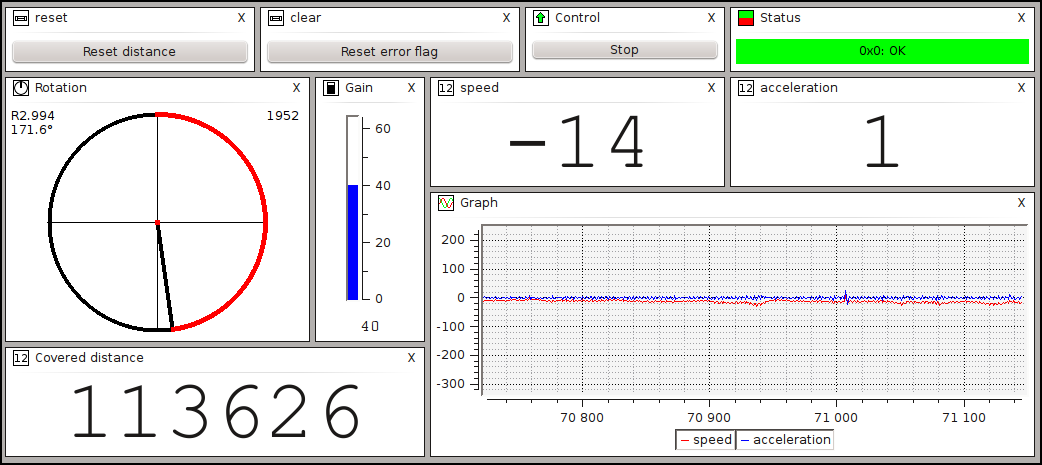
\includegraphics{img/enc_full.png}
\caption{Data from the encoder processed by analyzer}
\label{analyzer_all}
\end{center}
\end{figure}

\newpage
\begin{figure}[h]
\begin{center}
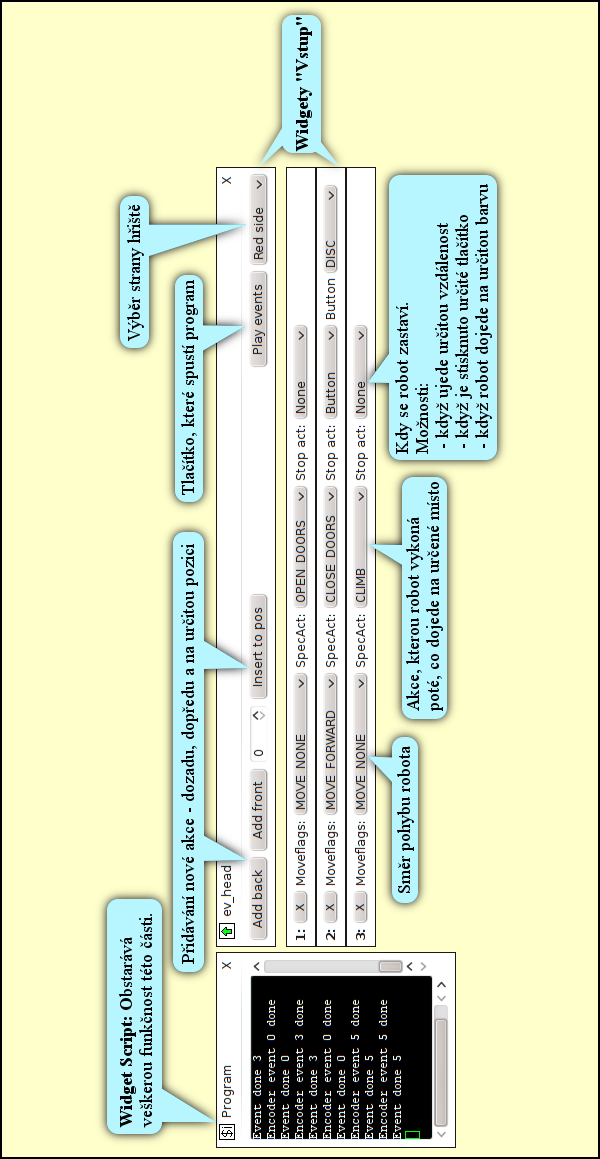
\includegraphics[width=750pt]{img/control_david.png}
\caption{Programming of robot's behavior in module \It{Analyzer}}
\label{david_ctrl}
\end{center}
\end{figure}
\end{landscape}

\pagestyle{plain}
\textheight=592pt
\textwidth=392pt
\newpage
\voffset = 0mm
\begin{figure}[H]
\begin{center}
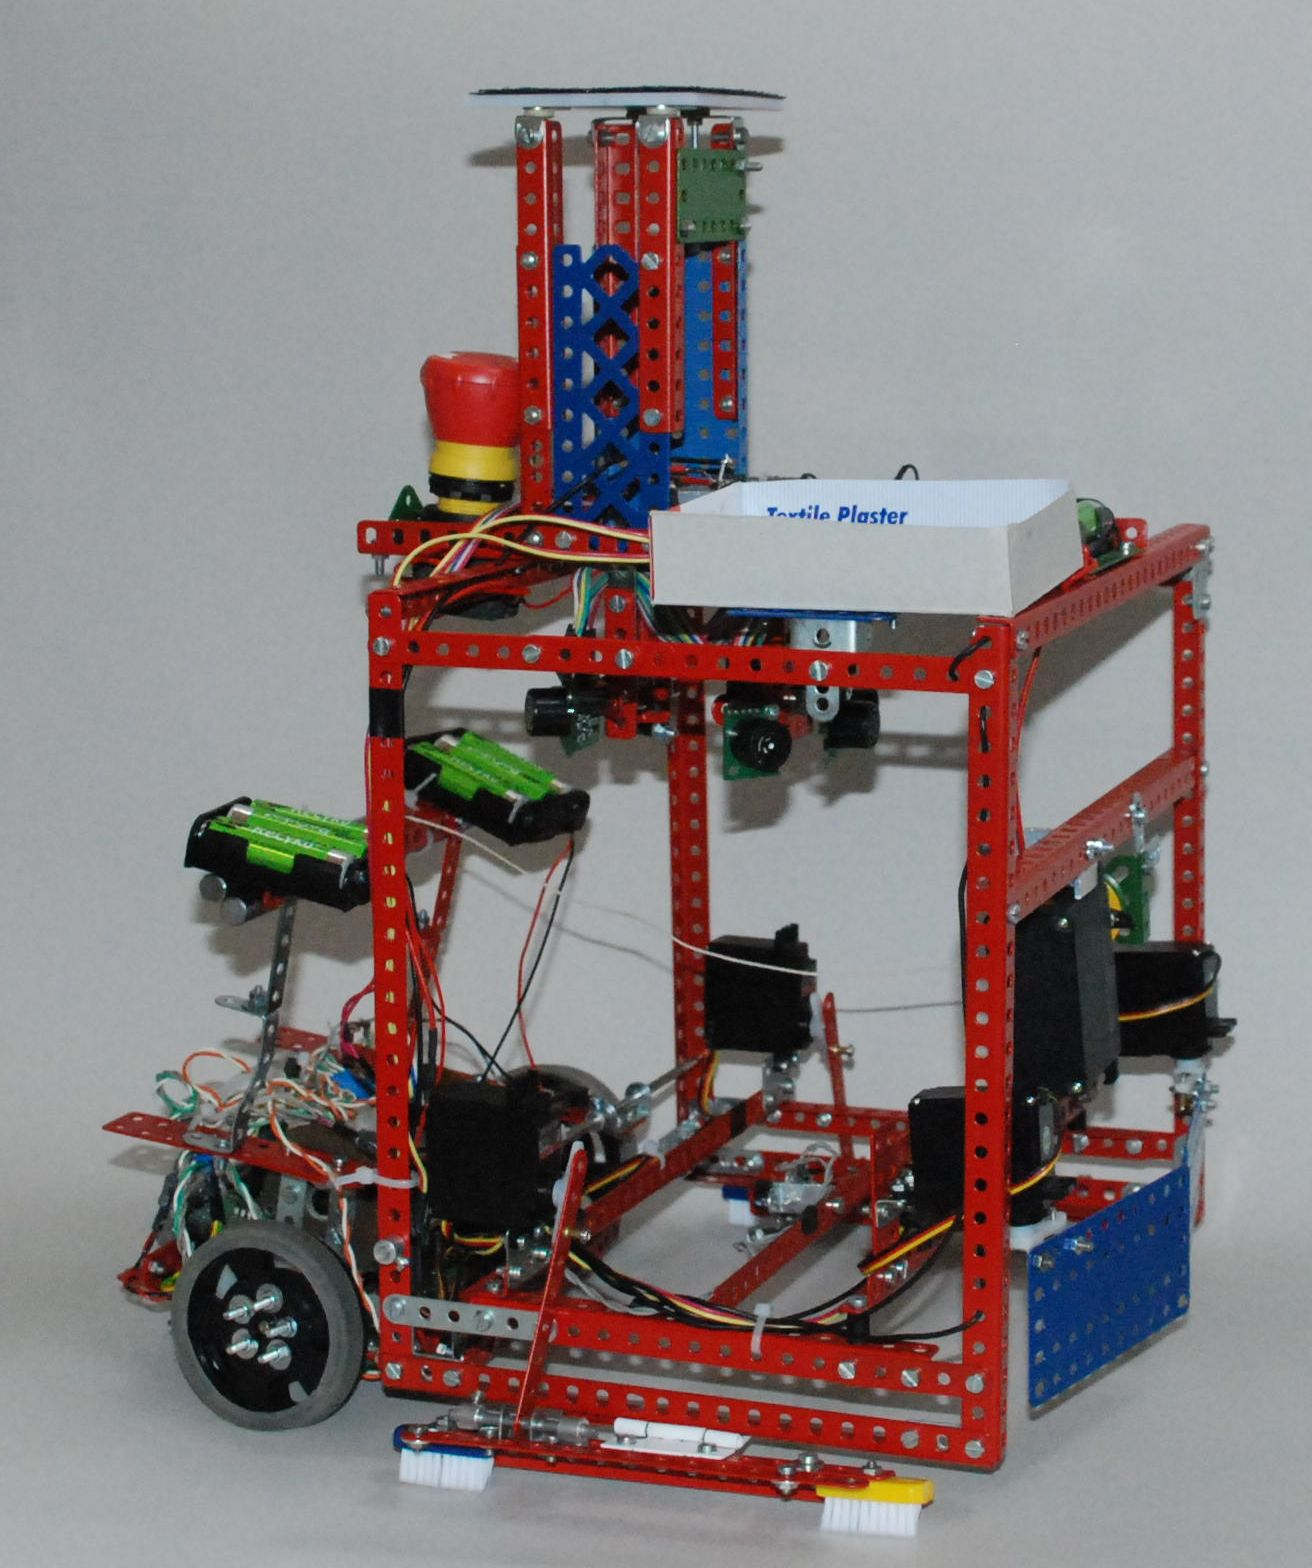
\includegraphics[width=\textwidth]{img/use_david_robot.jpg}
\caption{\It{David}, our robot, ended up on 4th place from the total of eleven robots in national round of Eurobot 2011 competition}
\label{david}
\end{center}
\end{figure}


\newpage
\section*{ATTACHMENT E:}
~
\addcontentsline{toc}{section}{ATTACHMENT E: List of images}
\listoffigures   % seznam obrázkù 

\end{document}